
\setcounter{chapter}{9-1}

\chapter{Convolutional Neural Networks}

    \subsection{Fully Connected Networks}

        Up to this point, we've focus on "\vocab{fully connected}" neural networks. 

        \begin{itemize}
            \item "Connected" refers to the "connection" between neurons in \textbf{adjacent} layers: one neuron provides the input for another.
        \end{itemize}

        \begin{figure}[H]
            \centering
            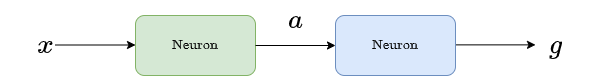
\includegraphics[width=70mm,scale=0.5]{images/nn_images/series_a.png}
            
            \caption*{These two neurons are connected.}
        \end{figure}

        Thus, "fully connected" means that every possible connection between pairs of neurons \orgg{exists}.\\
        
        \begin{definition}
            A \vocab{fully connected} (FC) layer is one where every \gren{input} neuron is connected to every \purp{output} neuron.

            The network layer only needs to be missing \redd{one} connection between neurons to not be fully connected.
        \end{definition}

        \miniex We compare two networks:

        \begin{figure}[H]
            \centering
            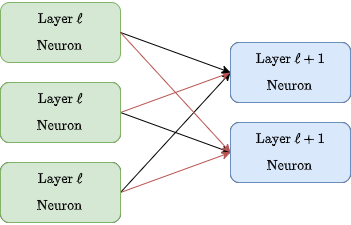
\includegraphics[width=50mm,scale=0.5]{images/convolutional_neural_networks_images/fully_connected.png}
            \qquad
            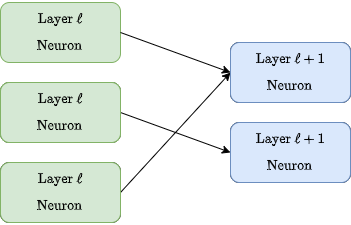
\includegraphics[width=50mm,scale=0.5]{images/convolutional_neural_networks_images/not_fully_connected.png}
            
            \caption*{The left network is fully connected: the right is not, having removed the red arrows.}
        \end{figure}

    \subsection{The drawbacks of fully-connected networks}
        
        The "fully connected" approach includes a \gren{weight} $w_{a,b}$ for every pair of input neuron $a$, and output neuron $b$.

        \begin{itemize}
            \item Each of these weights determines the \orgg{relationship} between our two neurons.
            \item In an FC settings, we're allowing for every possible pattern between pairs.
        \end{itemize}

        This is a very, very flexible model: any combination of patterns is possible. \\

        \begin{concept}
            Fully-connected networks are very useful when we \purp{know very little} about how to \gren{predict} our result.

            By including so many possible connections and patterns, we're open to lots of \purp{different models} we could try.

            \begin{itemize}
                \item This is especially helpful if we expect these relationship to be complex.
            \end{itemize}
        \end{concept}


        With a non-FC model, on the other hand, some connections have been severed. With this model, we're creating making some \textbf{assumptions} about which patterns \redd{don't} exist.
        
        \begin{itemize}
            \item \miniex If you think fact $A$ is irrelevant for computing fact $B$, you wouldn't include it in the equation.
            \item This is similar to how you want to exclude inputs that won't help you predict your output.\\
        \end{itemize}

        \begin{concept}
            \purp{Removing} a connection in a neural network is equivalent to saying, "I don't think this variable $a$ \orgg{should} affect this other variable $b$".
        \end{concept}

        This highlights a major \textbf{drawback} of fully connected networks: sometimes, it's inappropriate to allow for every possible connection.

        Having connections we don't need can cause plenty of problems:\\

        \begin{concept}
            \vocab{Fully-connected} networks come with some problems:

            \begin{itemize}
                \item Having many parameters can risk \purp{overfitting},
                \item Our model takes \gren{more time} to converge
                    \begin{itemize}
                        \item Both because it has to train \purp{more weights},
                        \item And because our model can get "distracted" by dead-end possibilities, that a simpler model wouldn't consider.
                    \end{itemize}
                \item It's often difficult to interpret \orgg{how} our neural network comes to the conclusions it does.
            \end{itemize}
        \end{concept}

        In this chapter, we'll introduce some more specific problems, and one model type that allows us to overcome these problems: \vocab{Convolutional Neural Networks}.

        \pagebreak

    \subsection{Intro to Image Processing}

        An excellent example for how FC neural networks can fail, is \vocab{image processing}.

        \miniex Facial recognition, self-driving vehicles, classifying the object in a picture

        Let's give it a try: suppose we have an image. For simplicity, it's black and white. We'll need to represent the \gren{brightness} of each pixel with a number.

        \begin{itemize}
            \item We'll use the most common range of values: the integers $[0,255]$.
        \end{itemize}


        \begin{figure}[ht]
            \begin{minipage}{.35\textwidth}
              \centering
              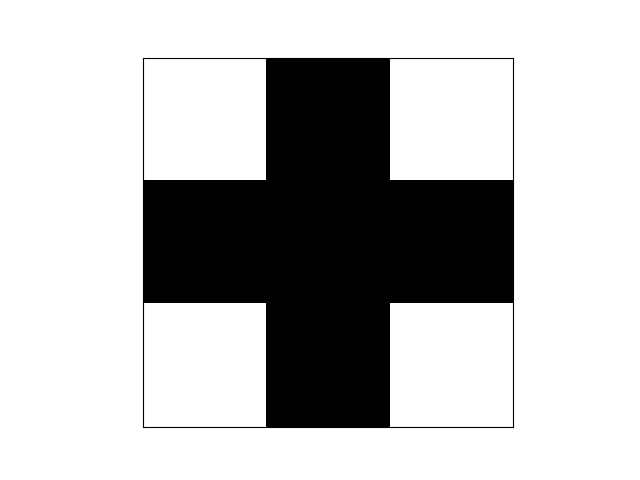
\includegraphics[width=.9\linewidth]{images/convolutional_neural_networks_images/crossgrid.png} 
            \end{minipage}
            \begin{minipage}{.3\textwidth}
                \centering
                $$\mathlarger{\mathlarger{\mathlarger{\implies}}}$$
            \end{minipage}
            \begin{minipage}{.1\textwidth}
                \centering
              \[
              \begin{bmatrix}
                  255 & 0 & 255 \\
                  0 & 0 & 0 \\
                  255 & 0 & 255
              \end{bmatrix}
              \]
            \end{minipage}
            \caption*{Our machine stores the "picture" on the right.}
        \end{figure}

        Our neural network takes a single $d \times 1$ vector as it's input. But right now, we have an $(r \times k)$ matrix. How do we solve that? With \purp{flattening}.\\

        \begin{definition}
            \vocab{Flattening} is the process of taking a \gren{matrix} of inputs, and transforming it into a single \purp{vector}.

            We usually do this by \orgg{concatenating} (combining consecutively) each row/column, in order.

            \begin{equation*}
                \begin{bmatrix}
                    \red{a} & \blu{b} \\ \red{c} & \blu{d}
                \end{bmatrix}
                \qquad \longrightarrow \qquad
                \begin{bmatrix}
                    \red{a} \\ \red{c} \\ \blu{b} \\ \blu{d}
                \end{bmatrix}
            \end{equation*}

            If the input is an $(r \times k)$ matrix, the result is an $(rk \times 1)$ vector.
        \end{definition}

        \miniex We can apply this to our data above.
            \note{We'll represent it with the transpose to save space.}

        \begin{equation}
            \begin{bmatrix}
                \red{255} & \pur{0} & \bro{255} \\
                \red{0} & \pur{0} & \bro{0} \\
                \red{255} & \pur{0} & \bro{255}
            \end{bmatrix}
            \qquad \longrightarrow \qquad 
            \begin{bmatrix}
                \red{255} & \red{0} & \red{255} & 
                \pur{0} & \pur{0} & \pur{0} & 
                \bro{255} & \bro{0} & \bro{255}
            \end{bmatrix}^T
        \end{equation}


        And so transform from $(3 \times 3)$ to $(9 \times 1)$.

        Looking at the image, or even the \textbf{matrix}, it's relatively easy to see the "\purp{cross}" pattern. 

        But, when we \vocab{flatten} it, those patterns immediately stop being obvious.

        \begin{itemize}
            \item We've lost information above which pixels are "\orgg{beside}" one another, for example.
                \note{Remember that we only took the row vector for visualization: they're stacked vertically based on column!}
        \end{itemize}

        Based on this, we'll find \textbf{two} main problems, that our CNNs will hopefully solve:

    \subsection{Spatial Locality}


        \textbf{First}: as we just mentioned, we need an idea of which pixels are close \gren{horizontally}.

        \begin{itemize}
            \item In fact, our network doesn't even care which pixels are \purp{above} each other \textbf{vertically}:\\
        \end{itemize}

        \begin{concept}
            \textit{Review from the Feature Representation chapter}
            
            The \vocab{order} we choose for elements in a vector \purp{doesn't} affect the behavior of our model, so long as we \textbf{consistently} use that order.

            This is because a linear model is a \gren{sum}:

            \begin{equation*}
                w^T a = \sum_i w_i a_i 
            \end{equation*}

            And sums are the same, regardless of \purp{order}.

            \begin{equation*}
                a+b=b+a \quad\implies\quad 
                \red{w_1a_1} + \blu{w_2a_2} = \blu{w_2a_2} + \red{w_1a_1} 
            \end{equation*}

            \subsecdiv

            \begin{itemize}
                \item We emphasize that the order does need to be \textbf{consistent} between data points.
            \end{itemize}
        \end{concept}

        \miniex Suppose $x_1$ represents height and $x_2$ represents weight.
            \begin{itemize}
                \item We could do either $[\text{weight},\text{height}]$ or $[\text{height},\text{weight}]$: it doesn't matter.
                    \note{BUT, we have to be \textbf{consistent} with which order we pick: otherwise, someone is measured as 180 feet tall, instead of 180 pounds.}
            \end{itemize}

        In other words, we could \purp{shuffle} the order of our pixels, and as long as we shuffled it the \textbf{same way} for all of our training data, it wouldn't matter to our \textbf{model}.

        \begin{itemize}
            \item This was fine for the above example, but it doesn't make sense for \textbf{image processing}, where each dimension is just a \textbf{pixel}:
        \end{itemize}

        Human vision works differently: we look for shapes, which are often made up of pixels \purp{near} each other: edges, points, corners, curves.

        \phantom{}

        \phantom{}

        \begin{itemize}
            \item In other words, we want to encode \textbf{local} information, across the physical \textbf{space} of our image. Thus, we call it \vocab{spatial locality}.
                \note{When we use "space" here, it's \textbf{different} from "latent space", or "input space". 
                
                \phantom{}
                
                Instead, we're talking about physical space: how physically \textbf{close} real things are, measured in \textbf{meters}, or in this case, \textbf{pixels}.}\\
        \end{itemize}

        \begin{definition}
            \vocab{Spatial locality} is the knowledge of which objects are \gren{close} in \purp{space} to each other.

            In an \orgg{image}, we might think of which pixels are "close" in that image.
                \begin{itemize}
                    \item Which pixels are next to, or on top of each other? How far apart? How are they "arranged"?
                \end{itemize}

            \subsecdiv

            \begin{itemize}
                \item This is a property we want to build into the structure of our CNNs.
            \end{itemize}
        \end{definition}

        \miniex If told that the white was blank space, and the black represented "objects", a human would have a concrete understanding of how these two images might be different:

        \begin{figure}[H]
            \centering
            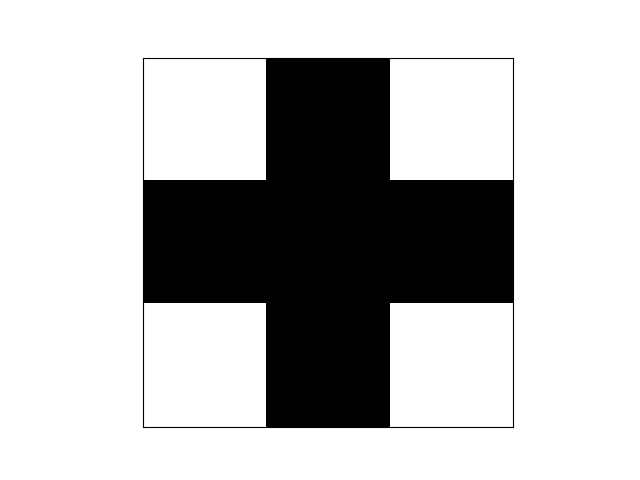
\includegraphics[width=50mm,scale=0.5]{images/convolutional_neural_networks_images/crossgrid.png}
            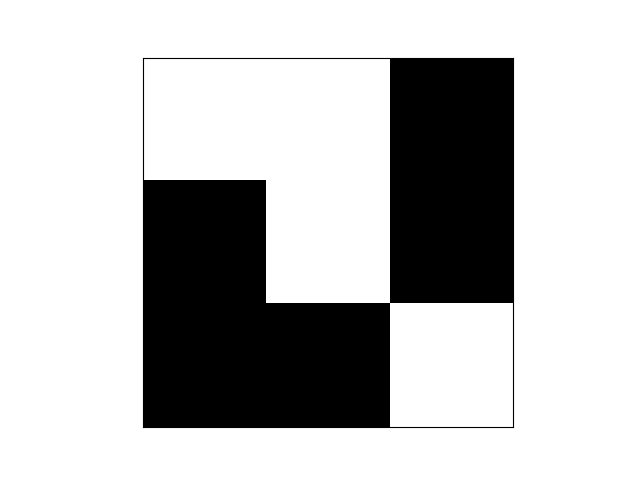
\includegraphics[width=50mm,scale=0.5]{images/convolutional_neural_networks_images/notcross_3.png}
            
            \caption*{The left image contains \textbf{one} object, while the right image contains \textbf{two} objects.}
        \end{figure}

        We figure this out based on which pixels are \textbf{touching} or not: a spatial property.

        \begin{itemize}
            \item The neural network would struggle to encode anything like that.
        \end{itemize}

        



        

        

    \subsection{Translation Invariance}

        A second problem is that, if the same \textbf{pattern} occupies different pixels, then it's completely new to the model.

        \begin{itemize}
            \item \miniex Suppose you have a cat on the left side of an image. You \purp{move} it to the right side of the image.
            \item A person would consider that image "\gren{almost the same}".
            \item But our FC NN does not: the cat is occupying a completely \purp{different set of pixels}, which have a completely separate set of weights attached.
        \end{itemize}

        So, our NN can't find structures that are \textbf{similar} across different parts of the input.

        Instead, we want a different behavior: we want our model to treat our input as the \textbf{same} (invariant), even if we move, or \textbf{translate} it.
            \note{Not language translation: "translation" as in "moving around in space".}

        \begin{itemize}
            \item Thus, we're looking for \vocab{translation invariance}.\\
        \end{itemize}

        \begin{definition}
            \vocab{Translation invariance} is the property of treating patterns as the \gren{same} even if we \purp{translate} them in space.

            In an \orgg{image}, we might want to recognize the same \gren{pattern} in two different \purp{positions} on the image.

            \begin{itemize}
                \item In other words, the pattern has "translated" from one of those positions, to the other.
            \end{itemize}

            \subsecdiv

            \begin{itemize}
                \item This is a property we want to build into our CNN.
            \end{itemize}
        \end{definition}

        \miniex In the following image, you would probably recognize "two crosses".

        \begin{figure}[H]
            \centering
            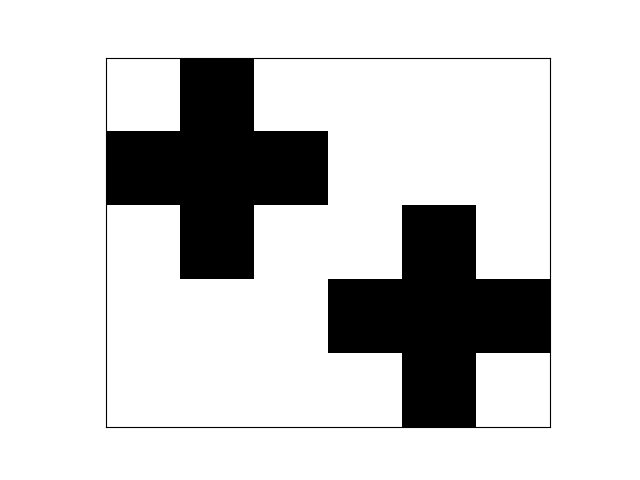
\includegraphics[width=70mm,scale=0.5]{images/convolutional_neural_networks_images/two_crosses.png}
            
            \caption*{We have two of the \textbf{same} object: just \textbf{translated} over.}
        \end{figure}

        But, because the top left pixels have separate weights from the bottom right pixels, the NN will react differently to each.

        Now that we've defined our problem, we can come up with a solution: \textbf{filters}.

        
\pagebreak

\section{Filters}

    \subsection{Motivating the Filter}

        So, we want a technique that handles both of these problems. 
    
        First, \vocab{translation invariance}: we want a calculation that can find the same pattern, in multiple locations.
    
        \begin{itemize}
            \item So, we'll apply the same calculation repeatedly, in \purp{multiple positions} on our image.

            \item We'll \gren{move} across our image, shifting to a new position each time we \orgg{scan} for that pattern.
        \end{itemize}

        \begin{figure}[H]
            \centering
            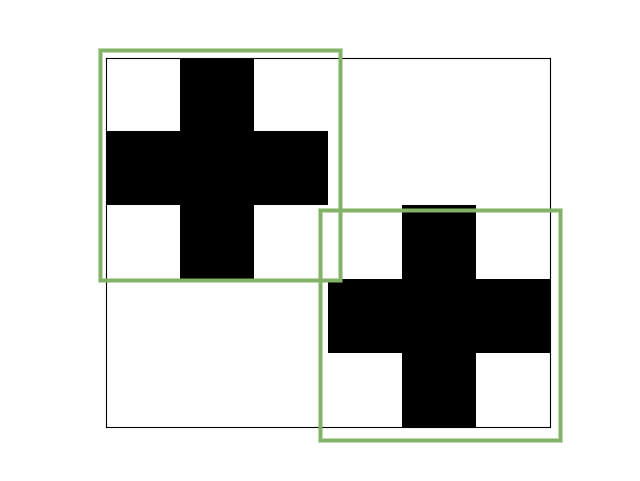
\includegraphics[width=70mm,scale=0.5]{images/convolutional_neural_networks_images/twocross_find.png}
            
            \caption*{As we "scan over" our image, we'll hopefully find both of our crosses separately.}
        \end{figure}

        Next, \vocab{spatial locality}: we want this calculation to encode \textbf{spatial} information.

        \begin{itemize}
            \item As we "scan" across our image, each computation will look for a particular "shape", or "\gren{pattern}" for our pixels.
            \item This pattern will be based on the \purp{relative location} of each pixel.
        \end{itemize}

        So, we're looking for a tool that repeatedly shifts (or \textbf{translates}) across our image, and looks for a spatial \textbf{pattern} in the image.

        \begin{itemize}
            \item \miniex Above, we would be looking for the "3x3 cross" pattern, and shift across rows/columns.
        \end{itemize}

        \begin{figure}[H]
            \centering
            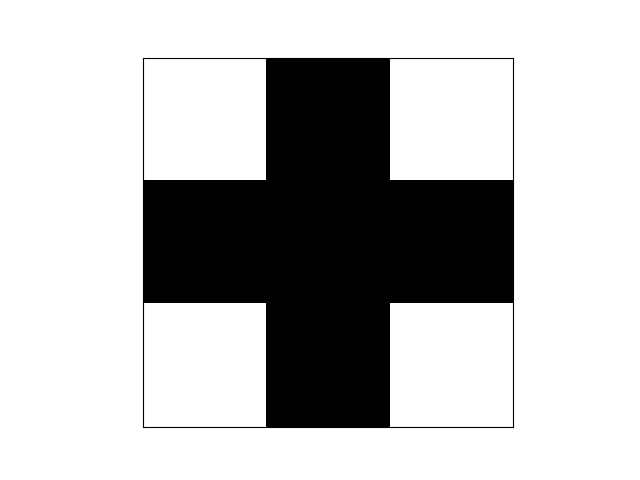
\includegraphics[width=40mm,scale=0.5]{images/convolutional_neural_networks_images/crossgrid.png}
            
            \caption*{This is the shape we are looking for at each position.}
        \end{figure}

        The tool in question is "looking" for a pattern. Another way to see it, is that it's \purp{filtering} out everything that doesn't match that pattern.
        
        \begin{itemize}
            \item Thus, we call it a \vocab{filter}.\\
        \end{itemize}

        \begin{concept}
            \vocab{Filters} handle both the problems of \gren{spatial locality} and \purp{translation invariance} at the same time.
        \end{concept}

        Notably, all of this works better if we keep our data in the \textbf{matrix} format, not the \textbf{flattened} one.

    \subsection{Windowing}

        We still need to figure out \textbf{how} we're going to find these patterns. 

        We've already established that our algorithm will look at a \gren{local} region of the image, and search for the pattern.

        To make life easier, we'll cut out a \purp{piece} of the image, and only compare that to the pattern. 

        \begin{figure}[H]
            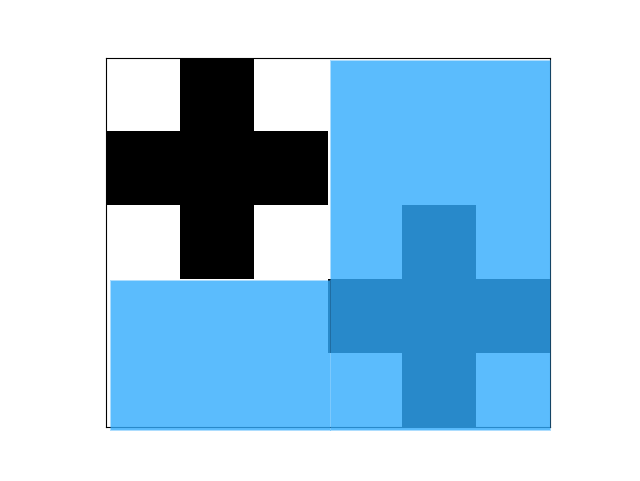
\includegraphics[width=45mm,scale=0.5]{images/convolutional_neural_networks_images/window.png}
            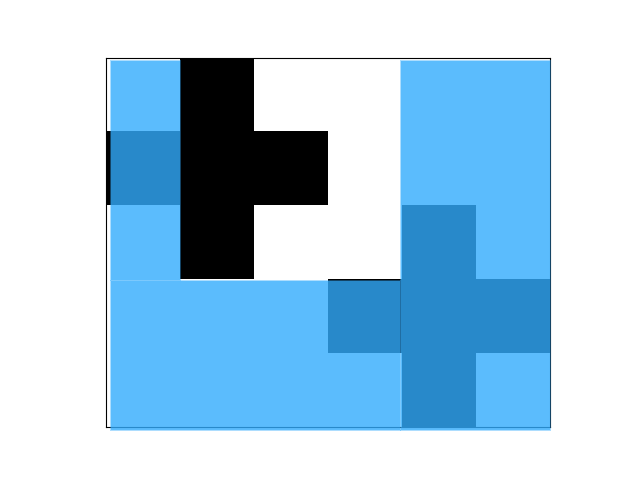
\includegraphics[width=45mm,scale=0.5]{images/convolutional_neural_networks_images/window2.png}
            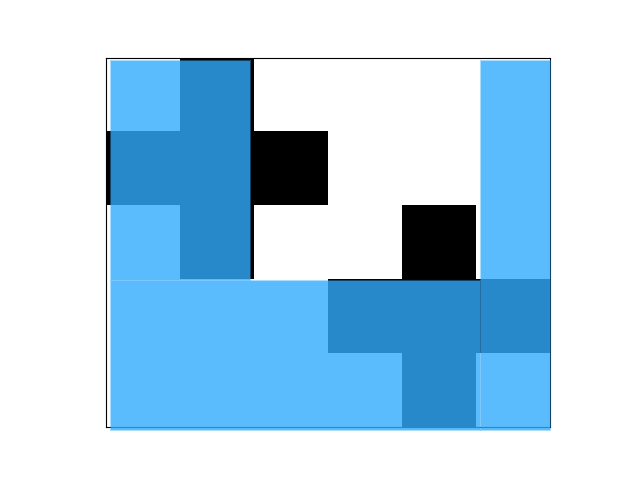
\includegraphics[width=45mm,scale=0.5]{images/convolutional_neural_networks_images/window3.png}
            
            \caption*{If we're viewing the top-left corner, we're ignoring everything else (blue-shaded). Then, we'll check the next position.}
        \end{figure}
        
        This region is the only part we "see", so we call it a \textbf{window}.\\

        \begin{definition}
            The \vocab{window} $v$ is the region of our image that we are, at a given moment, looking for our \purp{pattern} in.

            This is the region we are applying our \gren{filter} to.

            The window has the \orgg{same dimensions} as our filter, so we can compare them directly.

            \subsecdiv

            \begin{itemize}
                \item As we continue filtering, we'll repeatedly move our filter, shifting it to every valid position on the image.
            \end{itemize}
        \end{definition}
        


    \subsection{1-D case}

        To get going, we'll start with a 1D example.
            \note{This isn't just a simplification: when processing sound data, it'll be in a 1D form.}

        \begin{itemize}
            \item To make the math easier, we'll replace 0 and 255 with $+1$ and $-1$.
                \note{We've decided to make dark pixels +1, and bright pixels -1. Which convention we choose isn't important: it's just more easily visible.}
        \end{itemize}

        Suppose we're looking for "bright spots": pixels that are much brighter than their surroundings.


        \begin{figure}[ht]
            \begin{minipage}{.35\textwidth}
              \centering
              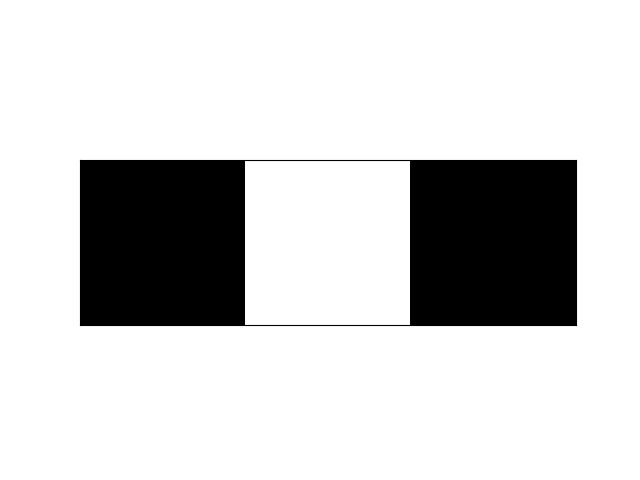
\includegraphics[width=.9\linewidth]{images/convolutional_neural_networks_images/1d_filter.png} 
            \end{minipage}
            \begin{minipage}{.3\textwidth}
                \centering
                $$\mathlarger{\mathlarger{\mathlarger{\implies}}}$$
            \end{minipage}
            \begin{minipage}{.1\textwidth}
                \centering
              \[
              \begin{bmatrix}
                  +1 & -1 & +1 \\
              \end{bmatrix}
              \]
            \end{minipage}
            \caption*{So, we're looking for something like this.}
        \end{figure}

        How do we find "bright spots", like this? Well, we want to find regions which are \textbf{similar} to our pattern.

        \begin{itemize}
            \item Our sequence is a vector, so we want to \purp{get the similarity between two vectors}.
            \item We have a tool for this! The \vocab{dot product} $a \cdot b$.\\
        \end{itemize}

        \begin{concept}
            \textit{Review from the Classification chapter}
            
            You can use the \vocab{dot product} between non-unit vectors to measure their "similarity" \purp{scaled by their magnitude}. 
            
            If two vectors are more \gren{similar}, they have a \gren{larger} dot product. 
            
            \begin{itemize}
                \item If angle$<90^{\circ}$ they are "similar": $\vec{a} \cdot \vec{b} > 0$
                
                \item If angle$>90^{\circ}$ they are "different": $\vec{a} \cdot \vec{b} > 0$
                
                \item If they are \orgg{perpendicular} (angle=$90^{\circ}$) to each other, $\vec{a} \cdot \vec{b} = 0$
            \end{itemize}
        \end{concept}

        So: as an approximation, the higher the dot product, the more similar they are!
            \note{This works extra well for something like an image, where the pixels have a restricted "range" of values: it's not as easy to get an extra-high dot product just because the magnitude are too large.}

       

        Now, we know what to do: we'll get the \textbf{dot product} between our window, and the \purp{filter}, to see how similar they are.

        \begin{itemize}
            \item If they're similar enough, then we found the pattern!\\
        \end{itemize}

        \begin{concept}
            To determine whether the window contains our pattern, we take the \vocab{dot product} between our \purp{window} $v$ and our \gren{filter} $f$.

            \begin{equation*}
                v \cdot f
            \end{equation*}

            The \gren{higher} the dot product, the \gren{more likely} that we have our pattern.

            \subsecdiv

            \begin{itemize}
                \item There's no exactly dot product value to be "sure" you've found your pattern: you have to choose your threshold based on context.
            \end{itemize}
        \end{concept}

        We'll show our example below.

    \pagebreak
    \subsection{1D Example}

        So, suppose we have our input image:

        \begin{figure}[ht]
            \begin{minipage}{.35\textwidth}
              \centering
              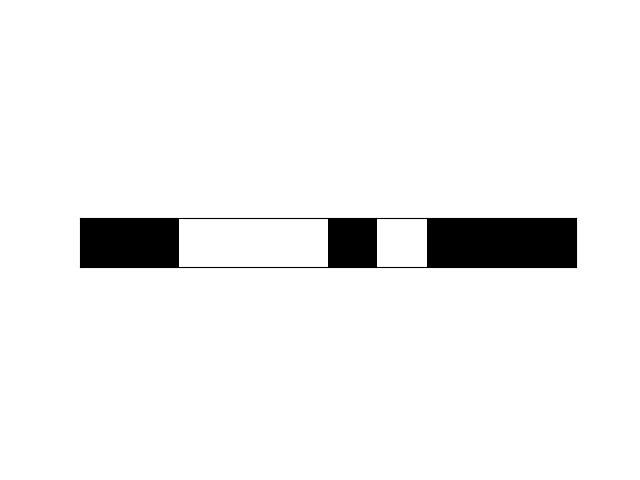
\includegraphics[width=.9\linewidth]{images/convolutional_neural_networks_images/1d_image.png} 
            \end{minipage}
            \begin{minipage}{.1\textwidth}
                \centering
                $$\mathlarger{\mathlarger{\mathlarger{\implies}}}$$
            \end{minipage}
            \begin{minipage}{.2\textwidth}
                \centering
              \[
              \begin{bmatrix}
                  \blu{+1}&\blu{+1}&\red{-1}&\red{-1}&\red{-1}&
                  \blu{+1}&\red{-1}&\blu{+1}&\blu{+1}&\blu{+1} \\
              \end{bmatrix}
              \]
            \end{minipage}
        \end{figure}

        Our filter is size 3 (3 elements), so we'll grab a window of 3 elements.

        \begin{figure}[ht]
            \begin{minipage}{.35\textwidth}
              \centering
              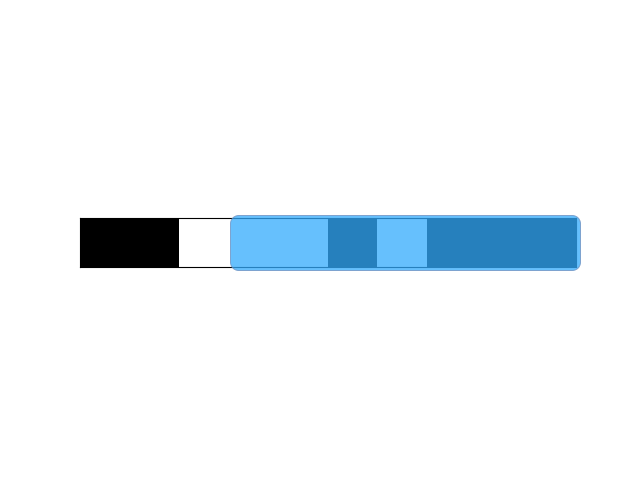
\includegraphics[width=.9\linewidth]{images/convolutional_neural_networks_images/1d_window1.png} 
            \end{minipage}
            \begin{minipage}{.1\textwidth}
                \centering
                $$\mathlarger{\mathlarger{\mathlarger{\implies}}}$$
            \end{minipage}
            \begin{minipage}{.2\textwidth}
                \centering
                \begin{equation*}
                    \begin{matrix}
                        \overbrace{
                        \begin{bmatrix}\blu{+1}&\blu{+1}&\red{-1}\end{bmatrix}
                        }^{\begin{bmatrix}
                          \blu{+1} & \red{-1} & \blu{+1}
                        \end{bmatrix}}
                        &
                        -1&-1&
                        +1&-1&
                        +1&+1&+1
                    \end{matrix}
                \end{equation*}
            \end{minipage}
            \caption*{We ignore everything after the first three elements.}
        \end{figure}

        We then compute the result:

        \begin{equation}
            \overbrace{
              \begin{bmatrix}
                  +1&+1&-1
              \end{bmatrix}
              }^{v}
              \qquad\implies \qquad
              \overbrace{\begin{bmatrix}
                    \blu{+1} \\ \red{-1} \\ \blu{+1}
                \end{bmatrix}}^{f} \cdot
                \overbrace{\begin{bmatrix}
                    \blu{+1} \\ \blu{+1} \\ \red{-1}
                \end{bmatrix}
                }^{v}
                \qquad=\qquad
                +1-1-1= \red{-1}
        \end{equation}

        

        This is our first filtering: we get -1. This is the first element of our output:

        \begin{equation}
            y = x \ast f =
            \begin{bmatrix}
                \red{-1} & ? & ? & ? & ? & ? & ? & ? 
            \end{bmatrix}
        \end{equation}
        
        We'll repeat for the rest of our 1d signal.
        
        \begin{figure}[H]
            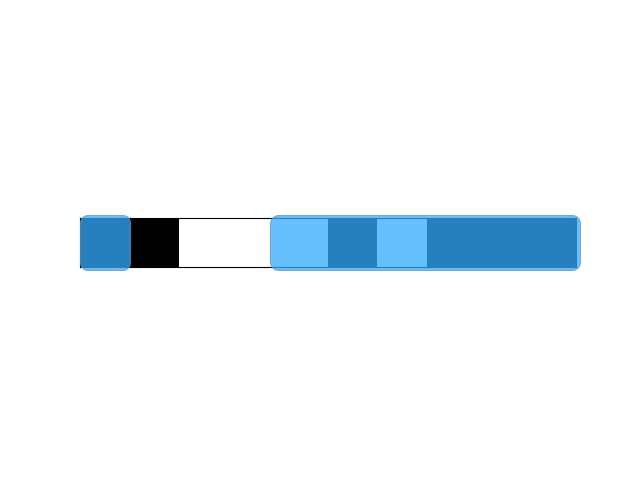
\includegraphics[width=45mm,scale=0.5]{images/convolutional_neural_networks_images/1d_window2.png}
            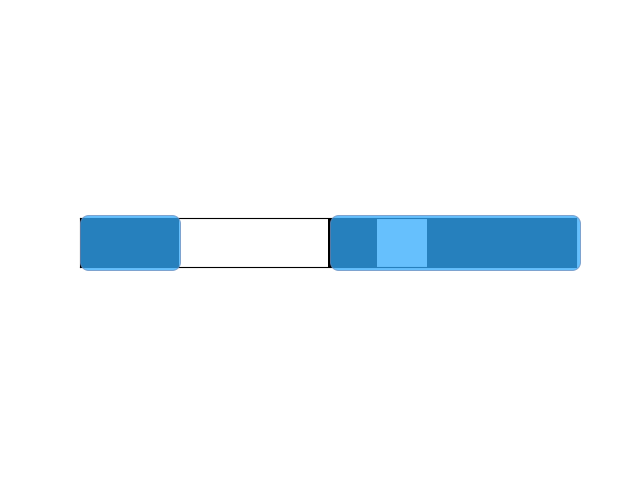
\includegraphics[width=45mm,scale=0.5]{images/convolutional_neural_networks_images/1d_window3.png}
            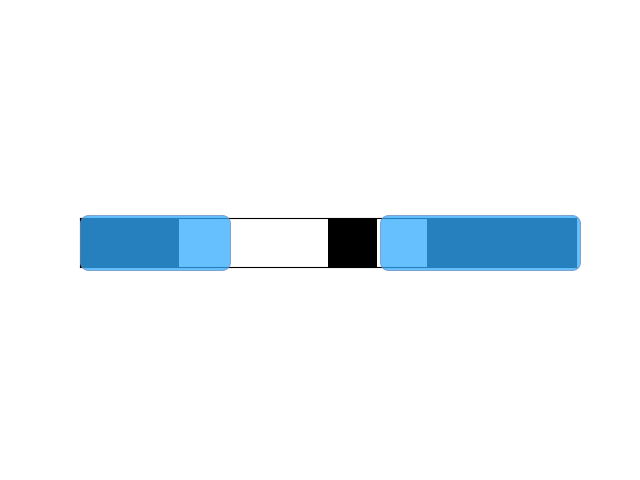
\includegraphics[width=45mm,scale=0.5]{images/convolutional_neural_networks_images/1d_window4.png}
        \end{figure}

        \begin{equation*}
            \begin{bmatrix}
                -1 & \mathbf{\blu{+1}} & \cdots & ?
            \end{bmatrix}
            \qquad\implies\qquad
            \begin{bmatrix}
                -1 & +1 & \mathbf{\red{-1}} & \cdots & ?
            \end{bmatrix}
            \qquad\implies\qquad
            \begin{bmatrix}
                -1 & +1 & -1 &\mathbf{\blu{+1}} & \cdots & ?
            \end{bmatrix}
        \end{equation*}

        This is \textbf{convolution}.

    \pagebreak

    \subsection{Convolution}
    
        Convolution simply applies our filter, at each position:\\

        \begin{concept}
            When filtering (doing \vocab{convolution}), the \gren{output} at the $\nth{i}$ index is given by having \purp{shifted} your window over from 0, $(i-1)$ times.

            \begin{itemize}
                \item The \orgg{indices} for our output usually start from index 1.
            \end{itemize}
        \end{concept}

        \miniex The last example above, ending at index 3, outputs +1 after shifting right 3 times.

        The result is a new vector:

        \begin{equation}
            y=x \ast f = 
            \begin{bmatrix}
                -1 & +1 & -1 & +1 & -3 & \org{+3} & -1 & +1
            \end{bmatrix}
        \end{equation}

        The pixel we have labelled in orange corresponds to the "bright spot" in our sequence:

        \begin{figure}[H]
            \centering
            
\includegraphics[width=80mm,scale=0.5]{images/convolutional_neural_networks_images/bright_spot_window.png}
        \end{figure}

        As we hoped, the "matching" pattern is the highest positive magnitude!

        With this, we've fully demonstrated 1-d \vocab{convolution}.\\

        \begin{definition}
            \vocab{Convolution} $x \ast f$ is the process of searching through a \purp{signal} $x$ for a particular \gren{pattern}, using a \gren{filter} $f$.

            \begin{itemize}
                \item The filter \purp{matches} the pattern we're looking for.
            \end{itemize}

            The convolution process follows the following steps:

            \begin{itemize}
                \item Taking a \gren{window} $v$ in the same shape as the filter, \gren{isolating} a section of your signal
                \item Applying a \purp{dot product}-like operation between your filter $f$ and your window $v$.
                \item \orgg{Sliding} your window, and \textbf{repeating}, until every output is computed.
            \end{itemize}

            \subsecdiv

            \begin{itemize}
                \item The $\nth{(i+1)}$ index is given for the dot product computed by shifting over $i$ times from index 1.
            \end{itemize}
        \end{definition}

        We call this a "\textbf{dot product-like operation}" to prepare us for \textbf{higher-dimensional} equivalents.

        We can even write this in formula terms. To represent \textbf{windowing}, we'll use python slices, with the same conventions.\\

        \begin{kequation}
            If we have \gren{signal} $x$, \purp{filter} $f$ of \purp{size} $k$, we can create a \orgg{window} $v_i$ by... 
            
            Starting at the \redd{leftmost} pixel, and shifting right by $i$ units:

            \begin{equation*}
                v_{\org{i+1}} = x \Big[ \pur{i}:\grn{i+k} \Big] =  
                \begin{bmatrix}
                    x_{i+1} \\ x_{i+2} \\ \vdots \\ x_{i+k}
                \end{bmatrix}
            \end{equation*}
            
            \begin{itemize}
                \item Note the subscript $v_{\org{i+1}}$: we start from $i=0$, and thus $v_1$.
                
            \end{itemize}

            This is used to create our \vocab{convolution} $y=x \ast f$:

            \begin{equation*}
                y_i = f \cdot v_i
            \end{equation*}
            
        \end{kequation}

        \note{The fact that $x$ is 1-indexed, but python slicing is 0-indexed, is the reason why $x[\red{i}:i+k]$ starts at $x_{\red{i+1}}$.}

        You might see a different version of indexing in some situations:
            \note{Like in the official notes!}\\

        \begin{clarification}
            Above, we used $i$ to give us the leftmost slice of our input.

            We did this because we assumed the \gren{leftmost} pixel would be assigned $i=0$.

            \begin{itemize}

                \item However, in some cases, the \purp{middle} pixel is assigned $i=0$: the pixels indices go equally positive or negative.
            \end{itemize}

            

            In which case, we would need to \orgg{replace} our slicing procedure above:

            \begin{equation*}
                x \Big[ \pur{i}:\grn{i+k} \Big] 
                \quad\longrightarrow\quad
                x \Big[ \red{(i- \lfloor k/2 \rfloor)}:\blu{(i+ \lfloor k/2 \rfloor)} \Big]
            \end{equation*}

            \begin{itemize}
                \item We use the floor operator $\lfloor x \rfloor$ so that we index correctly, by integers.
            \end{itemize}
        \end{clarification}

        One more thing: we need to be careful when we say we're doing "Convolution".\\

        \begin{clarification}
            In other fields, convolution requires \orgg{reversing the order} of your filter, before you apply it to your input.

            However, this is typically \textbf{not} the case in machine learning.
        \end{clarification}

        \pagebreak

    \subsection{Convolution Output Size}

        Something you might notice is that our output is \purp{smaller} than our input was.

        How much shorter? 2 elements: in general, the output of a convolution is \red{$k-1$} elements \textbf{shorter} than the input.
            \note{Where $k$ is, again, the size of our filter.}

        Why is this? We can see why, by focusing on the \gren{leftmost} element of our filter: we can only shift it until our vector ends.


        \begin{equation}
              \begin{matrix}
                  +1&+1&-1&-1&-1&
                  +1&-1&
                  \overbrace{
                  \begin{bmatrix}
                      \blu{+1}&\blu{+1}&\blu{+1}
                  \end{bmatrix} 
                  }^{\begin{bmatrix}
                      \blu{+1} & \red{-1} & \blu{+1}
                  \end{bmatrix}}
                  &\phantom{+1}&\phantom{+1}
              \end{matrix}
        \end{equation}

        But, our leftmost element hasn't reached the end of the vector: if it did, then the rest of the vector would be \orgg{sticking out}, with nothing to multiply with:

        \begin{equation}
              \begin{matrix}
                  +1&+1&-1&-1&-1&
                  +1&-1&\blu{+1}&\blu{+1}&
                  \overbrace{
                  \begin{bmatrix}
                      \blu{+1} & \phantom{?}? & \phantom{?}?
                  \end{bmatrix} 
                  }^{\begin{bmatrix}
                      \blu{+1} & \red{-1} & \blu{+1}
                  \end{bmatrix}}
              \end{matrix}
        \end{equation}

        When our leftmost position is as far right as we can go, there are $k-1$ positions remaining: the rest of the filter is "in the way".\\

        \begin{concept}
            For a length-$n$ input and a length-$k$ filter, \vocab{1d convolution} creates an output of size:

            \begin{equation*}
                n - (k-1)
            \end{equation*}
        \end{concept}

    \subsection{Padding}

        We don't necessarily want to be shrinking the size of our output. How do we solve this?

        Well, our equation above gives us two options: increase the input size, or decrease the filter size.

        \begin{itemize}
            \item Decreasing filter size is \textbf{restrictive}: the smaller the filter, the smaller the pattern we can search for.
            \item So, we'll just increase the size of our input.
        \end{itemize}

        We'll increase input size with \vocab{padding}: adding extra elements to the ends of our vector.

        \begin{itemize}
            \item Typically, we pad with 0's, to have the most neutral effect possible on our output.\\
        \end{itemize}
        
        

        \begin{definition}
            \vocab{Padding} is a technique for increasing the size of the output of convolution.

            To pad an input, you add filler values (usually 0's) to the \purp{edges} of the input vector.

            This allows the filter shift further in both directions.

            \subsecdiv

            A padding of $p$ adds $p$ values to \gren{both sides} of our input vector, transforming our $n$-sized input into a $n+2p$ sized input. Thus, our output size is:

            \begin{equation*}
                (n+2p) - (k-1)
            \end{equation*}

            Where $k$ is our filter size.
        \end{definition}

        \miniex Here's an example of \purp{zero-padding} with $p=2$:

        \begin{equation}
            \begin{bmatrix}
                1 & 2 & 3 & 4
            \end{bmatrix}
            \implies 
            \begin{bmatrix}
                \red{0} & \red{0} & 1 & 2 & 3 & 4 & \red{0} & \red{0}
            \end{bmatrix}
        \end{equation}

        Often, we select our padding size so the output size is the same as the input size: $2p=k-1$.

    \pagebreak

    \subsection{2D Filter}

        Now, we want to extrapolate this idea to higher dimensions: in particular, 2D, but this approach will work for any dimension.


        \begin{figure}[H]
            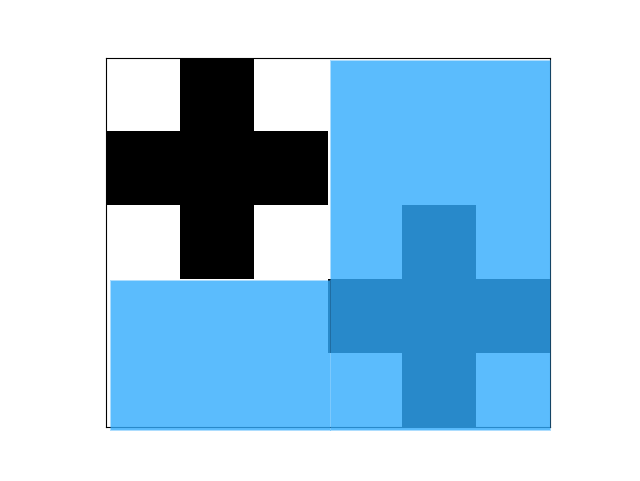
\includegraphics[width=45mm,scale=0.5]{images/convolutional_neural_networks_images/window.png}
            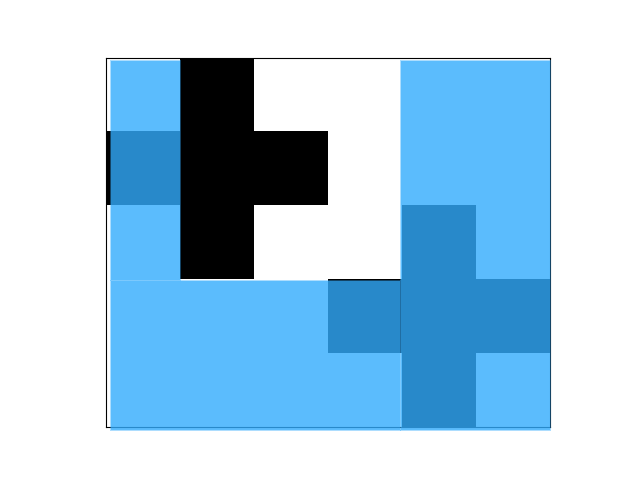
\includegraphics[width=45mm,scale=0.5]{images/convolutional_neural_networks_images/window2.png}
            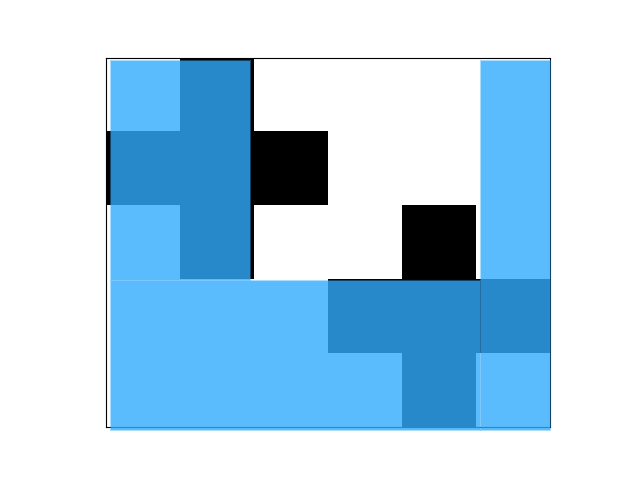
\includegraphics[width=45mm,scale=0.5]{images/convolutional_neural_networks_images/window3.png}
            
            \caption*{We're back to this example.}
        \end{figure}
        
        Let's review what we can already guess: first, we now have a 2-D pattern we're looking for, and a 2-D window cut out of our image.
        
        \begin{figure}[ht]
            \begin{minipage}{.35\textwidth}
              \centering
              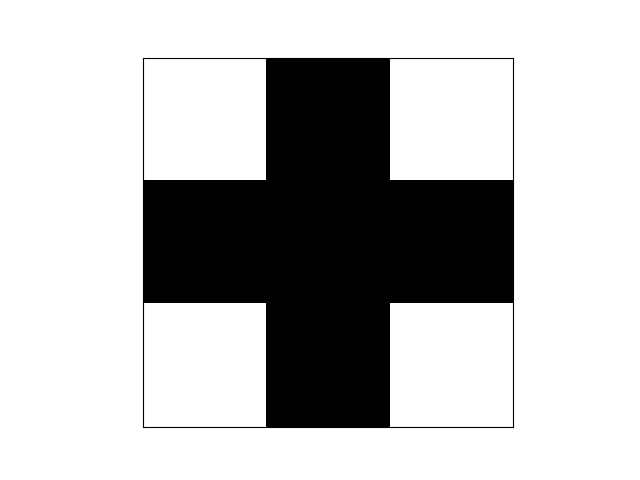
\includegraphics[width=.9\linewidth]{images/convolutional_neural_networks_images/crossgrid.png} 
            \end{minipage}
            \begin{minipage}{.3\textwidth}
                \centering
                $$\mathlarger{\mathlarger{\mathlarger{\implies}}}$$
            \end{minipage}
            \begin{minipage}{.1\textwidth}
                \centering
              \[
              \begin{bmatrix}
                  \red{-1} & \blu{+1} & \red{-1} \\
                  \blu{+1} & \blu{+1} & \blu{+1} \\
                  \red{-1} & \blu{+1} & \red{-1}
              \end{bmatrix}
              \]
            \end{minipage}
            \caption*{This is our filter.}
        \end{figure}
        
        \begin{figure}[ht]
            \begin{minipage}{.35\textwidth}
              \centering
              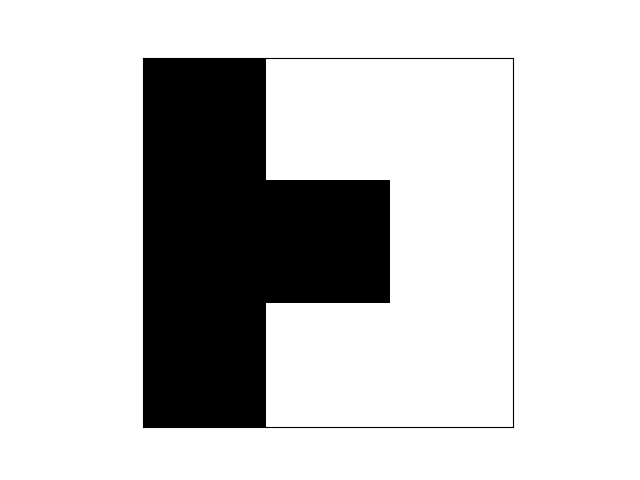
\includegraphics[width=.9\linewidth]{images/convolutional_neural_networks_images/window_2d.png} 
            \end{minipage}
            \begin{minipage}{.3\textwidth}
                \centering
                $$\mathlarger{\mathlarger{\mathlarger{\implies}}}$$
            \end{minipage}
            \begin{minipage}{.1\textwidth}
                \centering
              \[
              \begin{bmatrix}
                  \blu{+1} & \red{-1} & \red{-1} \\
                  \blu{+1} & \blu{+1} & \red{-1} \\
                  \blu{+1} & \red{-1} & \red{-1}
              \end{bmatrix}
              \]
            \end{minipage}
            \caption*{This is our window $w_{0,1}$: we've shifted over by one column.}
        \end{figure}

        How do we measure their similarity?

        \begin{equation}
            \begin{bmatrix}
                \red{-1} & \blu{+1} & \red{-1} \\
                \blu{+1} & \blu{+1} & \blu{+1} \\
                \red{-1} & \blu{+1} & \red{-1}
            \end{bmatrix}
            \text{ vs }
            \begin{bmatrix}
                \blu{+1} & \red{-1} & \red{-1} \\
                \blu{+1} & \blu{+1} & \red{-1} \\
                \blu{+1} & \red{-1} & \red{-1}
            \end{bmatrix}
        \end{equation}

        We measured similarity between vectors using the \orgg{dot product}.

        We can break our matrices up into vectors, by treating them as vectors of vectors.

        \begin{equation}
            \begin{bmatrix}
                \begin{bmatrix}
                    \red{-1} \\ \blu{+1} \\ \red{-1}
                \end{bmatrix} & 
                \begin{bmatrix}
                    \blu{+1} \\ \blu{+1} \\ \blu{+1}
                \end{bmatrix} & 
                \begin{bmatrix}
                    \red{-1} \\ \blu{+1} \\ \red{-1} 
                \end{bmatrix} 
            \end{bmatrix}
            \qquad\text{ vs } \qquad
            \begin{bmatrix}
                \begin{bmatrix}
                    \blu{+1} \\ \blu{+1} \\ \blu{+1}
                \end{bmatrix} & 
                \begin{bmatrix}
                    \red{-1} \\ \blu{+1} \\ \red{-1} 
                \end{bmatrix} & 
                \begin{bmatrix}
                    \red{-1} \\ \red{-1} \\ \red{-1} 
                \end{bmatrix} 
            \end{bmatrix}
        \end{equation}

        So, we can compare the similarity between the first vector in our \purp{filter}, and the first vector in the \gren{window} using the \textbf{dot product}.\\

        \begin{concept}
            If the $\nth{j}$ vector that makes up \purp{matrix $A$} is similar to the $\nth{j}$ vector that makes up \gren{matrix $B$}, then $A$ and $B$ are \orgg{similar}.

            \begin{equation*}
                \begin{matrix}
                    \overrightarrow{a} \approx \overrightarrow{d} \\\\
                    \overrightarrow{b} \approx \overrightarrow{e}\\\\
                    \overrightarrow{c} \approx \overrightarrow{f}
                \end{matrix}
                \implies 
                \begin{bmatrix}
                    \overrightarrow{a} & \overrightarrow{b} & \overrightarrow{c}
                \end{bmatrix}
                \approx
                \begin{bmatrix}
                    \overrightarrow{d} & \overrightarrow{e} & \overrightarrow{f}
                \end{bmatrix}
            \end{equation*}


        \end{concept}

        \begin{itemize}
            \item We'll repeat this process for each column.
        \end{itemize}

        \begin{equation}
            \overbrace{
                \begin{bmatrix}
                    \red{-1} \\ \blu{+1} \\ \red{-1}
                \end{bmatrix}
                \cdot 
                \begin{bmatrix}
                    \blu{+1} \\ \blu{+1} \\ \blu{+1}
                \end{bmatrix}
            }^{\text{Col 1}}
            \qquad+\qquad
            \overbrace{
                \begin{bmatrix}
                    \blu{+1} \\ \blu{+1} \\ \blu{+1}
                \end{bmatrix}
                \cdot 
                \begin{bmatrix}
                    \red{-1} \\ \blu{+1} \\ \red{-1} 
                \end{bmatrix}
            }^{\text{Col 2}}
            \qquad+\qquad
            \overbrace{
                \begin{bmatrix}
                    \red{-1} \\ \blu{+1} \\ \red{-1} 
                \end{bmatrix} 
                \cdot
                \begin{bmatrix}
                    \red{-1} \\ \red{-1} \\ \red{-1} 
                \end{bmatrix} 
            }^{\text{Col 3}}
        \end{equation}

        So, we've matched the $\nth{j}$ column of our window with the $\nth{j}$ column of our filter.

        \begin{itemize}
            \item And a dot product matches the $\nth{i}$ row of that window vector, with the $\nth{i}$ row of the filter vector.
        \end{itemize}

        That means, we're multiplying \purp{element-wise} across our matrix: the $(i,j)$ element of $f$ is multiplied by the $(i,j)$ element of $w$.\\

        \begin{definition}
            We introduce a \vocab{dot product generalization}, for a \orgg{matrix} (2-tensor):

            \begin{itemize}
                \item We compute it by multiplying \gren{element-wise}, then \purp{summing} all the elements.
            \end{itemize}

            \begin{equation*}
                A \cdot B = \sum_{i} \sum_j A_{ij} B_{ij}
            \end{equation*}

            This operation measures \orgg{similarity} between our two vectors.
        \end{definition}

        This allows us to do higher-dimensional convolution.

        \begin{figure}[H]
            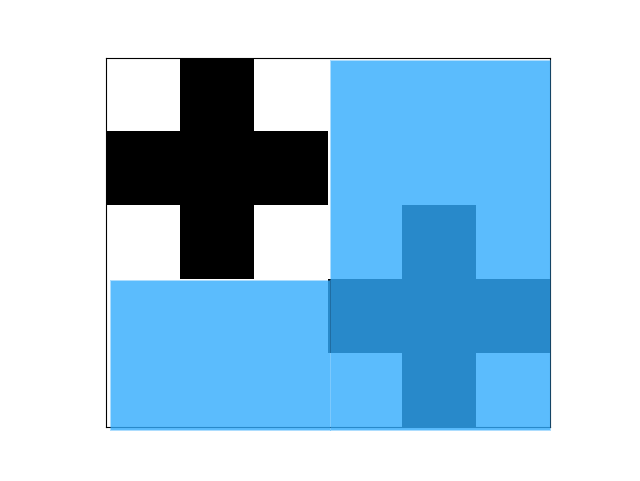
\includegraphics[width=45mm,scale=0.5]{images/convolutional_neural_networks_images/window.png}
            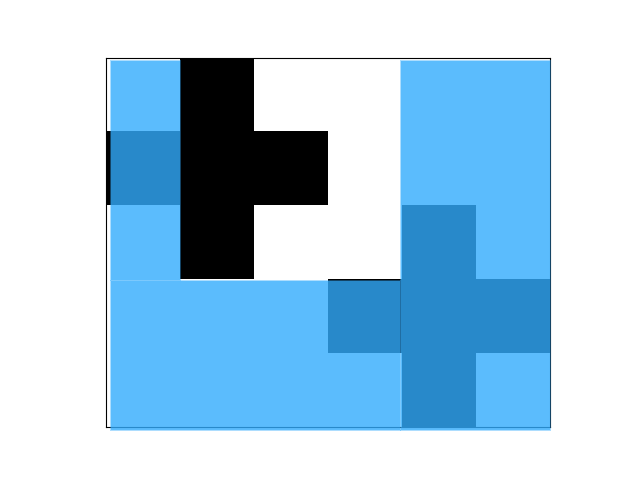
\includegraphics[width=45mm,scale=0.5]{images/convolutional_neural_networks_images/window2.png}
            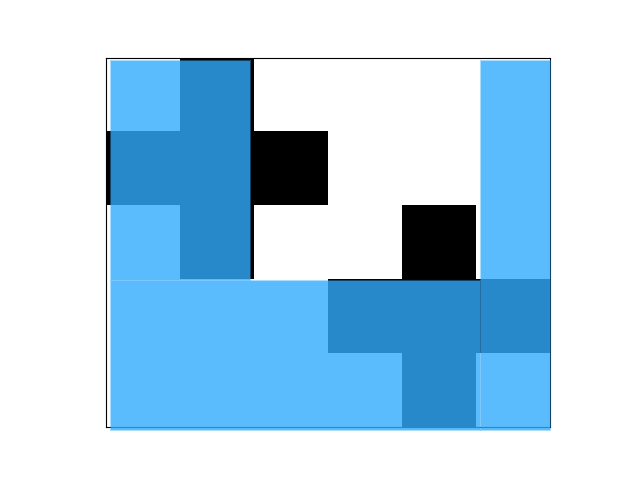
\includegraphics[width=45mm,scale=0.5]{images/convolutional_neural_networks_images/window3.png}
            
            \caption*{We're back to this example.}
        \end{figure}

    \subsection{2-D convolution}

        We'll need to shift around the image, in the same way that we did for the 1-d case.

        \begin{itemize}
            \item Before, we shifted over our \gren{window} (size $s$) across our \purp{input} (size $k$) by every possible position: this created $n-(k-1)$ outputs.
        \end{itemize}

        The process is the same here: we just need to shift along two axes.

        \begin{itemize}
            \item We'll need to consider every combination of shifting $i$ rows down, and $j$ rows right.
            \item In python, this is equivalent to a double for-loop: "for i in m, for j in n".\\
        \end{itemize}

        \begin{concept}
            For \vocab{2-D convolution}, we need to \gren{shift} our window along two axes.

            \begin{itemize}
                \item So, we have one window for each \purp{combination} of shifting $i$ rows down, $j$ columns right.
            \end{itemize}

            If we have an \gren{input} with an axis of length \grn{$n$}, and a \purp{filter} of size \purp{$k$}, that output axis has \orgg{length}

            \begin{equation*}
                (n+2p)-(k-1)
            \end{equation*}
            
            \begin{itemize}
                \item $k$ is typically the same on both of the 2d axes: it's usually \textbf{square}. 
            \end{itemize}
        \end{concept}

        \pagebreak

        \begin{remark*}
            Convolution was originally designed based on the way human eyes work: we use it to look for edges, and other distinct features in our vision.
        \end{remark*}
        
    \subsection{Dot Product Generalization}
        

        Later, we'll need to generalize this to higher dimensions: we'll review the higher-dimensional version of a matrix, the \vocab{tensor}:\\

        \begin{definition}
            \textit{Review from the Matrix Derivatives Chapter:}
            
            An \vocab{array} of objects is an \purp{ordered sequence} of them, stored together. 

            \begin{itemize}
                \item The most typical example is a \gren{vector}: an ordered sequence of \gren{scalars}.
            
                \item A \purp{matrix} can be thought of as a \gren{vector} of \gren{vectors}. For example: it could be a row vector, where every column is a column vector. 
            \end{itemize}
                
            Thus, a vector is a 1-d array, and a matrix is a 2-d array.
            
        \end{definition}
        
        We can extend this to any number of dimensions. We call this kind of generalization a \textbf{tensor}.\\
        
        \begin{definition}
            \textit{Review from the Matrix Derivatives Chapter:}
            
            In machine learning, we think of a \vocab{tensor} as a "\purp{multidimensional array}" of numbers.

            \begin{itemize}
                \item Each "dimension" is what we have been calling an "\purp{axis}".
                
                \item A tensor with $c$ axes is called a \vocab{$c$-Tensor}.
            \end{itemize}
            
        \end{definition}

        \miniex If we stacked a bunch of matrices in a box in 3-d, that would be a 3-tensor.

        To get element-wise multiplication, we'll need a way to index into tensors: we'll use numpy notation.\\

        \begin{notation}
            We want to \vocab{index} into a tensor $T$, with $n$ axes ("dimensions")
            
            We'll use indices $i_1,i_2,i_3, \cdots i_n$ to get an element:

            \begin{equation*}
                T \Big[ i_1,i_2,i_3, \cdots, i_n \Big]
            \end{equation*}
            
        \end{notation}

        Finally, we can show the dot-product generalization for tensors:
            \note{This is where python slicing really shines: it makes it easier to talk about grabbing an element from an unknown tensor.}\\

        \begin{definition}
            The \vocab{dot product generalization} for an arbitrary \orgg{$n$-Tensor}

            \begin{itemize}
                \item We compute it by multiplying \gren{element-wise}, then \purp{summing} all the elements.
            \end{itemize}
            

            \subsecdiv

            \begin{equation*}
                A \cdot B = \sum_{i_1,i_2,i_3, \cdots, i_n} 
                \red{A \Big[i_1,i_2,i_3, \cdots i_n  \Big]} \cdot 
                \blu{B \Big[i_1,i_2,i_3, \cdots, i_n \Big]}
            \end{equation*}
        \end{definition}


    \pagebreak 

    \subsection{Filter Banks}

        As we've shown, one filter produces one 2-d output: telling us where it "finds" or does not find the given pattern.

        But, typically, when doing complex image analysis, we don't just want \gren{one} filter. There are lots of different patterns we might be looking for.

        \begin{itemize}
            \item \miniex Rather than programming every larger shape \orgg{directly}, it might be easier to look for smaller edges.
            \item You'll need a \purp{different} filter for a vertical edge, or a horizontal edge, or a diagonal edge.
            
        \end{itemize}

        \begin{figure}[H]
            \centering
            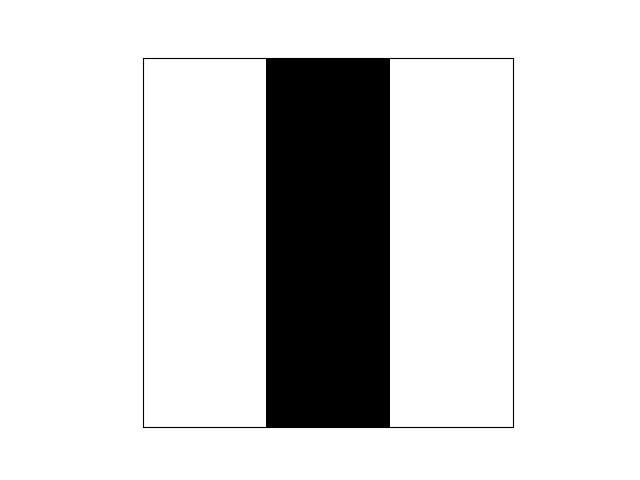
\includegraphics[width=30mm,scale=0.5]{images/convolutional_neural_networks_images/vertical_edge.png}
            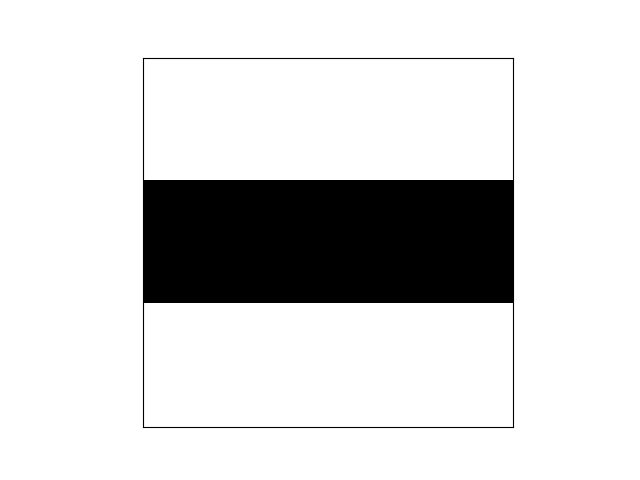
\includegraphics[width=30mm,scale=0.5]{images/convolutional_neural_networks_images/horizontal_edge.png}
            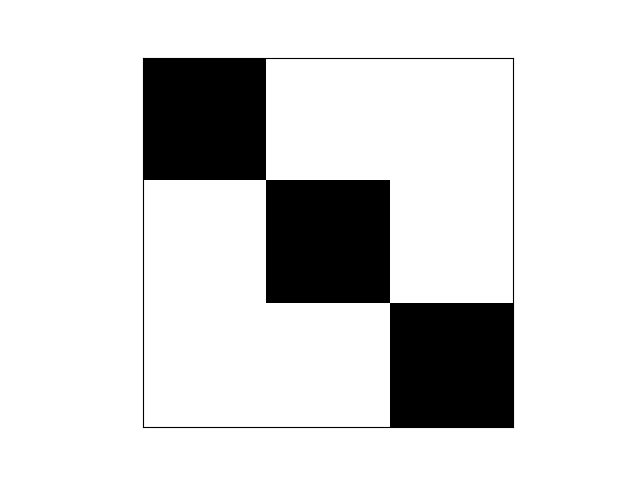
\includegraphics[width=30mm,scale=0.5]{images/convolutional_neural_networks_images/diag_1.png}
            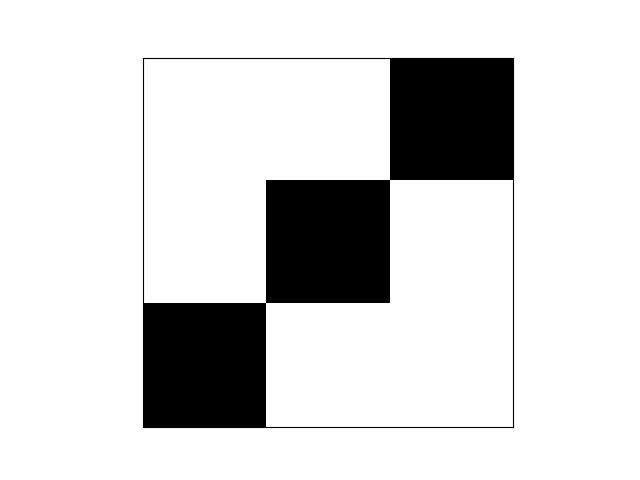
\includegraphics[width=30mm,scale=0.5]{images/convolutional_neural_networks_images/diag_2.png}
            
            \caption*{All four of these might be useful for the same image.}
        \end{figure}

        In practice, you almost always want to look for more than one pattern at the same time, in an image. 

        We'll store all of these filters together. Suppose we have $m$ of these filters: each filter has size $k$.
        
        \begin{itemize}
            \item Each is a 2d matrix, so we'll \textbf{stack} them in the third dimension.
            \item This creating a \vocab{tensor} in the shape $(k \times k \times m)$.
        \end{itemize}

        

        This collection is called a \vocab{filter bank}.\\

        \begin{definition}
            A \vocab{filter bank} is a collection of all of our $(k \times k)$ filters stacked into a \purp{3-tensor}.

            \begin{itemize}
                \item Thus, if we have $m$ of these filters, the \purp{shape} is $(k \times k \times m)$.
            \end{itemize}

            These filters are all applied to our image in \orgg{parallel}: meaning, each is applied to the original image, and each creates a separate output.
        \end{definition}

        \miniex We might, for example, combine the two following filters:
            \note{It's difficult to visualize a 3d thing like this, so if this looks strange, don't worry.}

        \begin{figure}[ht]
            \begin{minipage}{.35\textwidth}
              \centering
              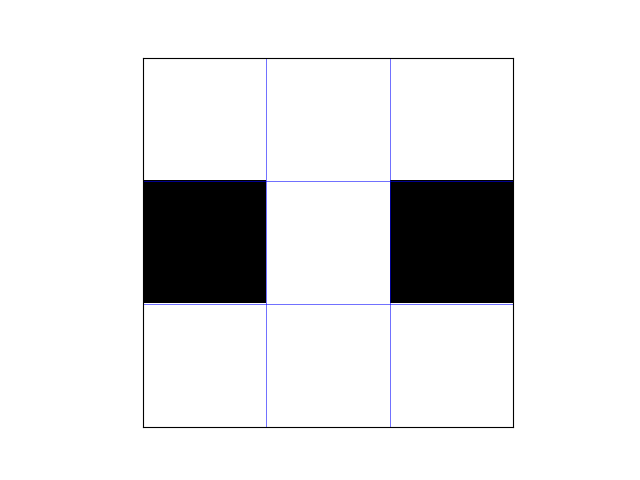
\includegraphics[width=.6\linewidth]{images/convolutional_neural_networks_images/filterbank_1.png}
              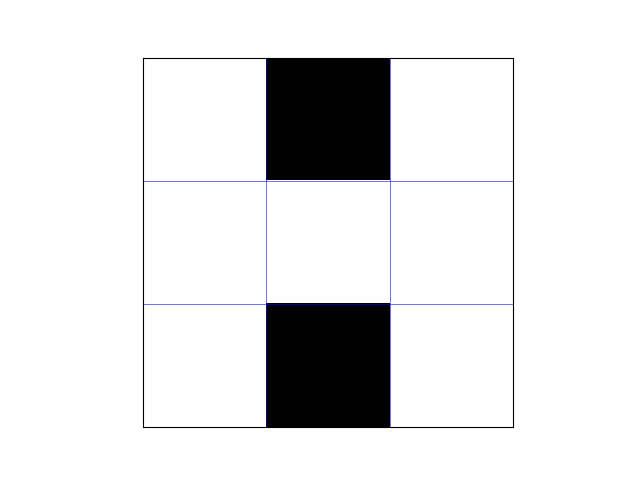
\includegraphics[width=.6\linewidth]{images/convolutional_neural_networks_images/filterbank_2.png}
            \end{minipage}
            \begin{minipage}{.3\textwidth}
                \centering
                $$\mathlarger{\mathlarger{\mathlarger{\implies}}}$$
            \end{minipage}
            \begin{minipage}{.1\textwidth}
                \centering
                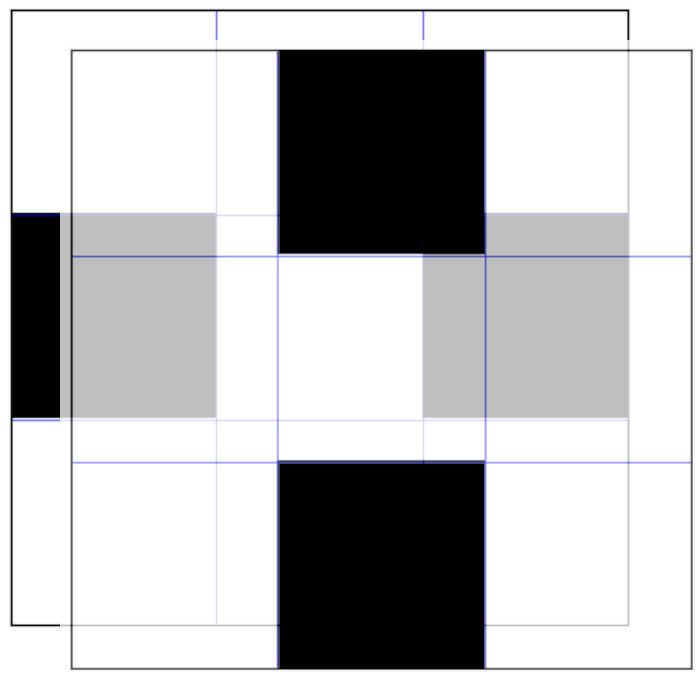
\includegraphics[width=30mm,scale=0.5]{images/convolutional_neural_networks_images/filterbank_k2.png}
            \end{minipage}
            \caption*{Now, we have a very simple filter bank.}
        \end{figure}

        \begin{clarification}
            This $(k \times k \times m)$ object could be a \orgg{filter bank}, but it could \purp{also} be a single \gren{3-tensor filter}, for a 3-tensor input.

            Why would our \gren{input} be a 3-tensor? We'll see why in a bit.
        \end{clarification}

        So, we'll use each of these filters, and \purp{convolve} them with the input. Each creates a separate output stored in a separate \gren{channel}.\\

        \begin{concept}
            A \vocab{channel} is the output of convolving \gren{one filter} with our \purp{image}.

            In a 2d image problem, one channel is a \orgg{matrix}.
        \end{concept}

        Each filter creates one channel. So, in order to depict all of our channels of output, we'll need another 3-tensor.\\

        \begin{concept}
            Suppose we have our 2d input.

            If we have $m$ filters in our \purp{filter bank}, we end up with $m$ \gren{channels} in our output.
        \end{concept}

        \begin{itemize}
            \item \miniex Here, we'll apply two filters: one detecting vertical lines, one detecting horizontal lines. It'll create two channels of output.
        \end{itemize}

        \begin{figure}[H]
            \centering
            \begin{minipage}{.2\textwidth}
                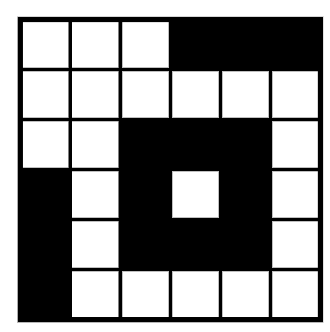
\includegraphics[width=20mm,scale=0.5]{images/convolutional_neural_networks_images/input_image.png}
            \end{minipage}
            \begin{minipage}{.2\textwidth}
                \centering
                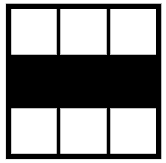
\includegraphics[width=10mm]{images/convolutional_neural_networks_images/horizontal_filter.png}
                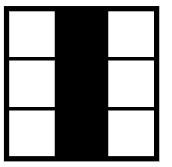
\includegraphics[width=10mm]{images/convolutional_neural_networks_images/vertical_filter.png}
                \caption*{$\mathlarger{
            \mathlarger{\mathlarger{\mathlarger{\mathlarger{\implies}}}}}$}
            \end{minipage}
            \begin{minipage}{.2\textwidth}
            \qquad
                $\begin{matrix}
                    ? & ? & ?  \\
                    ? & ? & ?  \\
                    ? & ? & ?  
                \end{matrix}$
            \end{minipage}
            \caption*{We're applying a simple filter bank to the image on the left.}
        \end{figure}

        \begin{figure}[ht]
            \begin{minipage}{.35\textwidth}
              \centering
              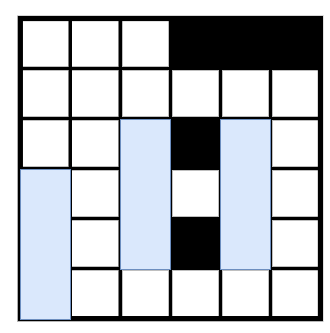
\includegraphics[width=.35\linewidth]{images/convolutional_neural_networks_images/vertical_detection.png}
            \end{minipage}
            \begin{minipage}{.25\textwidth}
                \centering
                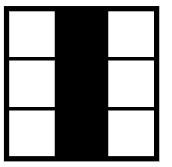
\includegraphics[width=.25\linewidth]{images/convolutional_neural_networks_images/vertical_filter.png}
                \caption*{$\mathlarger{\mathlarger{\mathlarger{\mathlarger{\mathlarger{\implies}}}}}$}
            \end{minipage}
            \begin{minipage}{.35\textwidth}
                \centering
                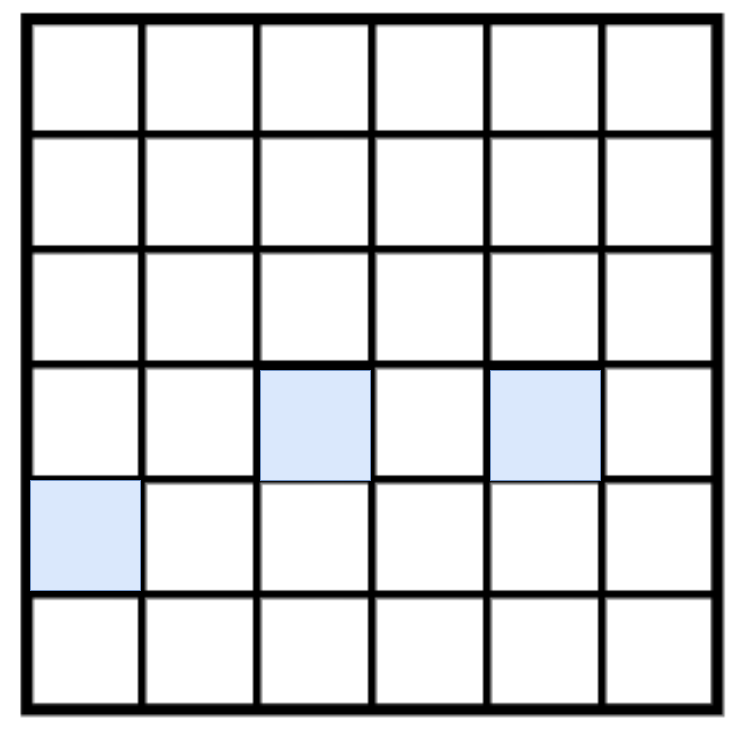
\includegraphics[width=.35\linewidth]{images/convolutional_neural_networks_images/vertical_channel.png}
            \end{minipage}
            \caption*{Our vertical detection.}
        \end{figure}

        \begin{figure}[ht]
            \begin{minipage}{.35\textwidth}
              \centering
              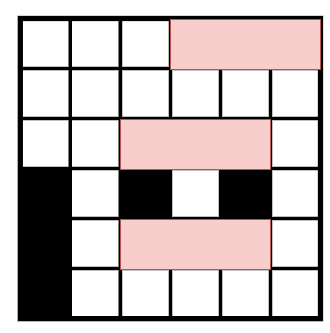
\includegraphics[width=.35\linewidth]{images/convolutional_neural_networks_images/horizontal_detection.png}
            \end{minipage}
            \begin{minipage}{.25\textwidth}
                \centering
                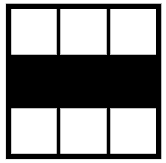
\includegraphics[width=.25\linewidth]{images/convolutional_neural_networks_images/horizontal_filter.png}
                \caption*{$\mathlarger{\mathlarger{\mathlarger{\mathlarger{\mathlarger{\implies}}}}}$}
            \end{minipage}
            \begin{minipage}{.35\textwidth}
                \centering
                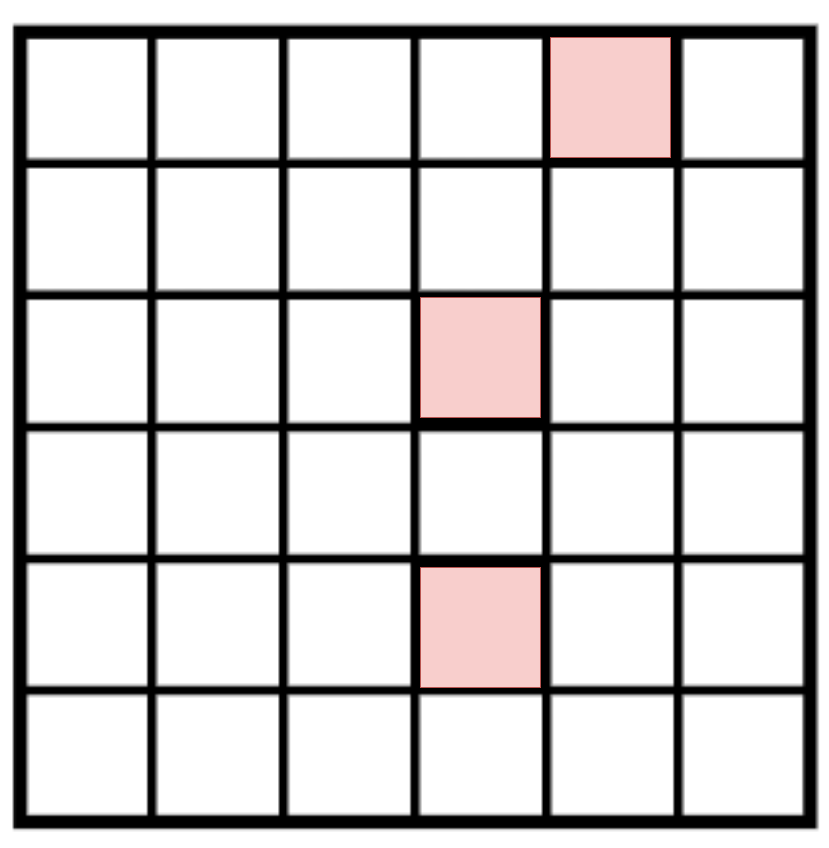
\includegraphics[width=.35\linewidth]{images/convolutional_neural_networks_images/horizontal_channel.png}
            \end{minipage}
            \caption*{Our horizontal detection.}
        \end{figure}

        Together, these create two channels:
  

        \begin{figure}[ht]
            \centering
            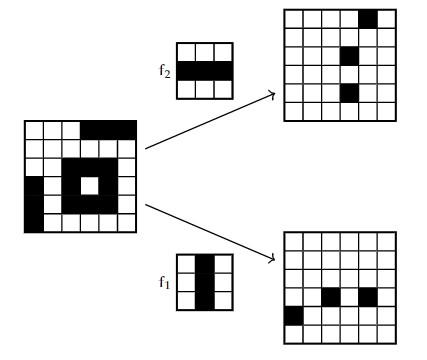
\includegraphics[width=.5\linewidth]{images/convolutional_neural_networks_images/two_channels.png}
        \end{figure}

    \pagebreak

    \subsection{Tensor Filters}

        Now, we have two different channels in our output. What do we do with this result?

        Each of our filters was designed to find a particular \gren{pattern}: you could say it represents one "\purp{perspective}" on the data.

        \begin{itemize}
            \item Our two filters above think about the data in terms of vertical lines, and horizontal lines.
        \end{itemize}

        We want to \purp{combine} those perspectives to get useful information. 

        \miniex A "square" is made out of two vertical lines, and two horizontal lines.

        \begin{figure}[H]
            \centering
            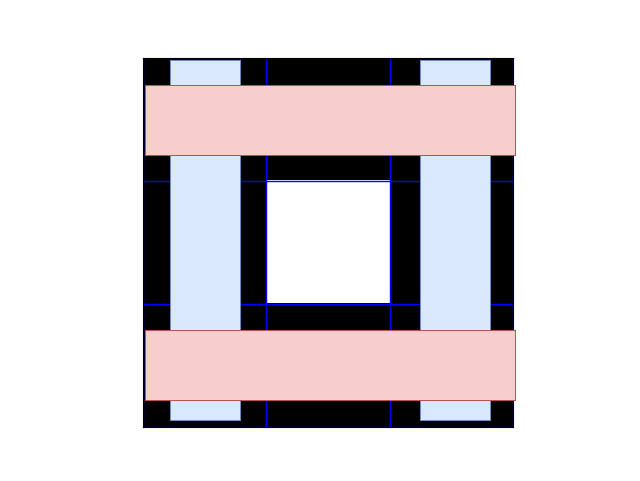
\includegraphics[width=.3\linewidth]{images/convolutional_neural_networks_images/square_marked.png}
        \end{figure}

        That means we want to find two \textbf{vertical} lines, and two \textbf{horizontal} lines: each on the opposite side of our center pixel.

        \begin{itemize}
            \item This is a kind of \textbf{pattern} we could search for, but it's a pattern across \purp{two channels}.
            \item That means that we need a filter occupying \textbf{multiple channels}. 
        \end{itemize}

        Let's see the pattern we want to see on each channel:

        \begin{figure}[ht]
            \begin{minipage}{.35\textwidth}
              \centering
              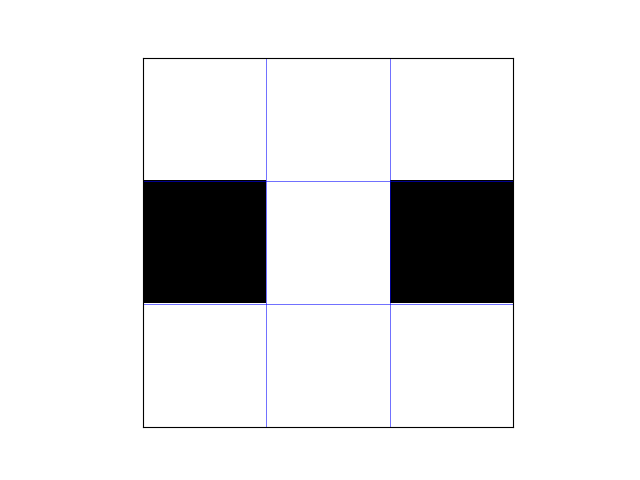
\includegraphics[width=.45\linewidth]{images/convolutional_neural_networks_images/filterbank_1.png}
              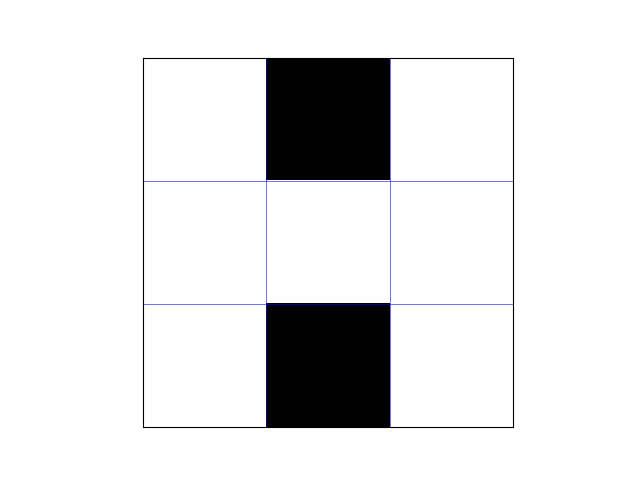
\includegraphics[width=.45\linewidth]{images/convolutional_neural_networks_images/filterbank_2.png}
            \end{minipage}
            \begin{minipage}{.25\textwidth}
                \centering
                \caption*{$\mathlarger{\mathlarger{\mathlarger{\mathlarger{\mathlarger{\implies}}}}}$}
            \end{minipage}
            \begin{minipage}{.45\textwidth}
                \centering
                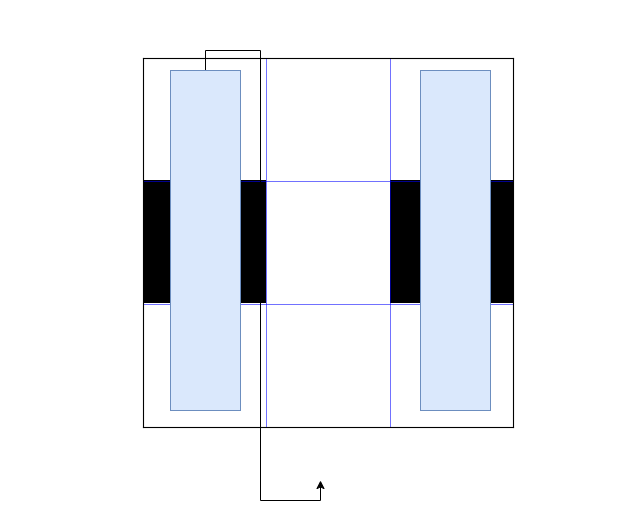
\includegraphics[width=.45\linewidth]{images/convolutional_neural_networks_images/filterbank_vertical.png}
              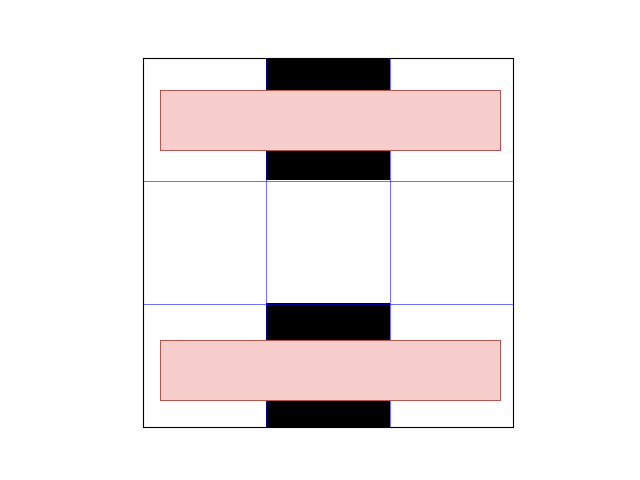
\includegraphics[width=.45\linewidth]{images/convolutional_neural_networks_images/filterbank_horizontal.png}
            \end{minipage}
            \caption*{The right side shows what each pixel on the filter "represents".}
        \end{figure}

        We want both at the same time, so we create a \vocab{3d filter}:

        \begin{figure}[H]
            \centering
            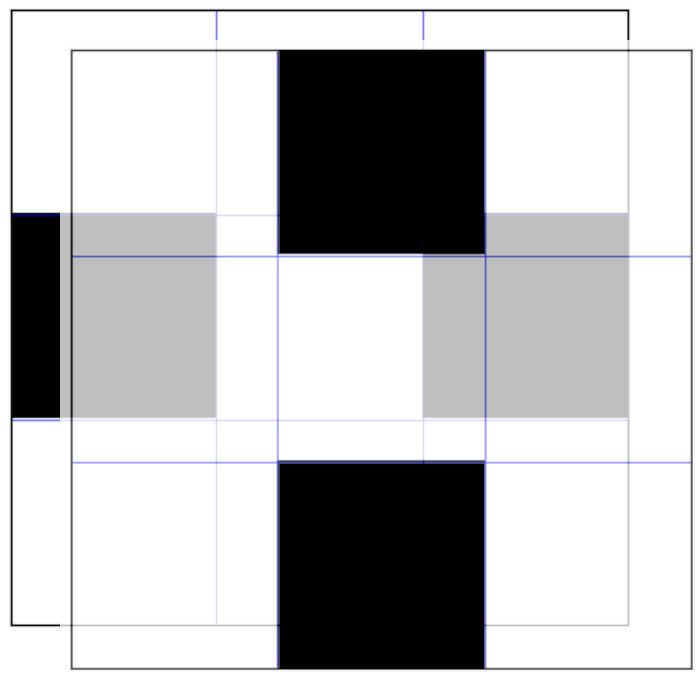
\includegraphics[width=.3\linewidth]{images/convolutional_neural_networks_images/filterbank_k2.png}
            \caption*{This looks like our 3d filter bank, of \textbf{2 filters}. But in this case, it's a \textbf{single} 3d filter.}
        \end{figure}

        Let's apply this trick to the two channels we designed earlier: we're going to find "donut" patterns in the original image.
            \note{Couldn't we have just used a donut-shaped filter in the first place, and then only need one filter?
            
            Yes, but this is useful for demonstrative purposes. }

        \begin{figure}[ht]
            \centering
            \includegraphics[width=.5\linewidth]{images/convolutional_neural_networks_images/two_channels.png}
            \caption*{Here's our previous work, finding vertical and horizontal lines.}
        \end{figure}

        \begin{figure}[ht]
            \centering
            \includegraphics[width=.7\linewidth]{images/convolutional_neural_networks_images/two_layer_conv.png}
            \caption*{And now, we'll combine those lines to create a square.}
        \end{figure}

        Look at that: our result is, we \textbf{only} get an output where there's a hollow square in the \textbf{original} input!

        We've found a more interesting pattern, using a \purp{second layer} of convolution.

    \subsection{Tensor Filters: All channels}

        When we introduce a \gren{3-tensor filter}, we could imagine not only moving across the rows and columns of the input, as we convolve, but also the \orgg{channels}.

        \begin{itemize}
            \item Thus, we would need to shift our filter along 3 axes.
        \end{itemize}

        However, in practice, we frequently \purp{avoid} this: instead, our tensor filter tends to have the \gren{same number of channels} as the input tensor.

        \begin{itemize}
            \item If they have the same number of channels, then there's no space to "shift" along the third axis.
            \item That means that the output of this filtering is a single matrix again!
                \note{Technically, it's a tensor with the shape $(m \times n \times 1)$. The last dimension being 1 is why it's effectively a "matrix".}\\
        \end{itemize}

        \begin{concept}
            Typically, our \vocab{3-tensor filters} occupy \purp{all channels of the input}.

            \begin{itemize}
                \item So, if the input is shape $(a \times b \times c)$, the filter has the shape $(k \times k \times c)$.
            \end{itemize}

            That means that our 3-tensor filter creates a \gren{matrix} as its output, when we do convolution.
        \end{concept}

        This allows us to add more tensor filters: our filter bank can contain multiple 3-tensors, and each one creates one channel of the output.
            \note{This means that our filter bank is a 4-tensor......... don't think too hard about it.}\\

        \begin{concept}
            Often, we use several \vocab{3-tensor} filters: each one occupies \gren{all of the input channels} at the same time.

            \begin{itemize}
                \item And each one outputs a single \textbf{matrix}.
            \end{itemize}

            That means that we can stack these 3-tensors into a \textbf{filter bank}: this object is now a \textbf{4-tensor}.

            \begin{itemize}
                \item When we apply this \orgg{4-tensor filter bank} to our \gren{3-tensor input}, we get a \purp{3-tensor output}.
            \end{itemize}
        \end{concept}
        

    \subsection{Convolution is Linear}

        You might have noticed that, above, we could have \textbf{replaced} all of our filters with a single, donut-shaped filter.

        \begin{itemize}
            \item We didn't do this, so we could \textbf{demonstrate} how convolution works conceptually.
        \end{itemize}

        This is possible because convolution, being entirely made out of \textbf{multiplication} and \textbf{addition}, is a \vocab{linear} operation.

        So, two consecutive convolutions are "\textbf{compressible}" to one, just like linear layers.\\

        \begin{concept}
            Machine learning "\vocab{convolution}", or "cross-correlation", is a \gren{linear} operation.

            \begin{itemize}
                \item Here, we'll summarize linearity as "\purp{multiplying} our variables $x$ by scalars (in this case, weights from $f$), and \gren{adding} the result together.

                \begin{equation*}
                    v \cdot f = \overbrace{\sum_i}
                    ^{\begin{matrix}
                        \text{Summing} \\ \text{Variables}
                    \end{matrix}} 
                    \overbrace{v_if_i}
                    ^{\begin{matrix}
                        \text{Scalar} \\ \text{Product}
                    \end{matrix}}
                \end{equation*}
            \end{itemize}

            In fact, as we'll see later when doing backprop, \gren{convolution} between $x$ and $f$ can be represented using a particular \purp{matrix multiplication}.
        \end{concept}

        This isn't a problem in practice because we'll add ReLU and max-pool layers in between: both are \purp{nonlinear}.
            \note{We haven't discussed max-pool yet.}

        That said, a "convolutional layer" is not a "linear layer":\\

        \begin{clarification}
            While convolution is \gren{linear}, \redd{a convolutional layer is different from a linear layer}.
    
            Why is that?
    
            Because convolution is a very \purp{restricted} kind of linear: 
    
            \begin{itemize}
                \item In \vocab{convolution}, we use the \gren{same filter} for every dot product -- every operation uses the same weights in $f$.
                \item In a \textbf{fully connected}, "\vocab{linear layer}", every input-output pair has a \purp{separate, independent} weight, that can be tuned freely.
            \end{itemize}

            \subsecdiv

            You could think that a FC/"linear" layer refers to the broadest, \orgg{least-restricted} kind of linear transformation:

            \begin{itemize}
                \item Every possible linear relationship is allowed.
            \end{itemize}

            You could also think of it as the "simplest" linear layer: it makes the least assumptions.
        \end{clarification}

    \subsection{RGB colors (\redd{Optional})}

        One quick concern, that's more pragmatic: all of our images, so far, have been in black-and-white.

        How do real pictures create color? Using the \vocab{RGB} system: each pixel has a certain brightness of red, green, and blue.

        \begin{itemize}
            \item So, to represent the pixel output, you need \purp{three} numbers: a brightness in the $[0,255]$ range for each color.
        \end{itemize}

        That means that our input isn't a 2d image: it's actually 3d.\\

        \begin{concept}
            If we're using \redd{R}\gren{G}\vocab{B} color instead of black-and-white (BW), each pixel requires \purp{3 values} to represent the \gren{brightness} of each color.

            Thus, if our BW image had the shape $(m \times n)$, our RGB image has the shape $(m \times n \org{\times 3})$: we use a \redd{3-tensor} to store the extra information about color.

            \begin{itemize}
                \item Thus, our filters have to be 3d filters, as well.
            \end{itemize}
        \end{concept}

    \pagebreak

    \subsection{Adding Convolution to our Neural Networks}

        So, we've developed a complete system for \purp{convolution}, using \textbf{filter banks}. How do we apply this to \vocab{machine learning}?

        Well, thankfully, our neural networks are very \textbf{modular}: 

        \begin{itemize}
            \item Each FC layer is \gren{self-contained}, and \purp{abstracted}: when we depict it this way, we only care about the input and output dimensions.
                \note{By "self-contained" and "abstracted", we mean that we can hide the contents of the layer, while still having a useful representation.}
        \end{itemize}

        \begin{figure}[H]
            \includegraphics[width=\textwidth]{images/nn_images/all_layers.png}
            \caption*{We've broken our model into "modules" that we could swap out: this representation doesn't acknowledge the weights, or the structure.}
        \end{figure}

        So, it's not too different if, instead of a \textbf{fully-connected} layer, we were to have a \vocab{convolutional} layer.\\

        \begin{concept}
            A \vocab{convolutional layer} can be inserted into a neural network by placing it \gren{between} two other layers.

            \begin{itemize}
                \item You just need to make sure the input/output have the right \purp{dimensions}.
            \end{itemize}
        \end{concept}

        Let's figure out how to \textbf{implement} that, while thinking in familiar NN terminology.

        Convolution is based on your window and filter. 
        
        \begin{itemize}
            \item Your \gren{window} is simply given by your input tensor, and how far you've \gren{shifted}.
            \item Your \purp{filter} is what really defines your convolution: it chooses the \purp{pattern} you're looking for.
        \end{itemize}

        

        \begin{figure}[ht]
            \begin{minipage}{.35\textwidth}
              \centering
              \includegraphics[width=.6\linewidth]{images/convolutional_neural_networks_images/crossgrid.png} 
            \end{minipage}
            \begin{minipage}{.3\textwidth}
                \centering
                $$\mathlarger{\mathlarger{\mathlarger{\implies}}}$$
            \end{minipage}
            \begin{minipage}{.1\textwidth}
                \centering
              \[
              \begin{bmatrix}
                  \red{-1} & \blu{+1} & \red{-1} \\
                  \blu{+1} & \blu{+1} & \blu{+1} \\
                  \red{-1} & \blu{+1} & \red{-1}
              \end{bmatrix}
              \]
            \end{minipage}
        \end{figure}

        So, we'll focus on the filter: this is how we determine the behavior of our convolutional layer.

        \begin{itemize}
            \item This is similar to how our \purp{weight} matrix $W$ is used to configure a layer of our FC NN.
            \item So, we say that our convolutional layer is defined by the \purp{weights} in our filters.
        \end{itemize}

        Note that we say \gren{filters}: we already established that we can use multiple filters. If we do, our output will have multiple channels.\\

    

        \begin{definition}
            Our \vocab{convolutional layer} is entirely determined by the \purp{weights} we choose for our \gren{filter bank}.

            \begin{itemize}
                \item For \orgg{each filter} in our filter bank, we'll also include a single \purp{offset}, or bias term.
            \end{itemize}

            \subsecdiv

            Suppose that, in the 1d case, we have a window of size $k$, for our input $x$. Our window shifted by $i$, is labelled $v_{i+1}$. 

            \begin{equation*}
                v_{\org{i+1}} = x \Big[ \pur{i}:\grn{i+k} \Big] =  
                \begin{bmatrix}
                    x_{i+1} \\ x_{i+2} \\ \vdots \\ x_{i+k}
                \end{bmatrix}
            \end{equation*}

            
            We've chosen weights for our filter $f$, with a bias term $f_0$. The $\nth{i}$ element of our \gren{output} for that filter is:

            \begin{equation*}
                y_i = v_i \cdot f + f_0
            \end{equation*}
        \end{definition}

        \miniex If we have a 2d filter of length $k$, then we need $k^2$ weights, and 1 bias. We have $k^2+1$ parameters.

        \begin{equation}
            f = 
            \begin{bmatrix}
                W_{11} & W_{12} & \cdots & W_{1n} \\
                W_{21} & W_{22} & \cdots & W_{2n} \\
                \vdots & \vdots & \ddots & \vdots \\
                W_{m1} & W_{m2} & \cdots & W_{mn} \\
            \end{bmatrix}
            \qquad
            f_0 = W_{0}
        \end{equation}

        Each convolutional layer has one filter bank, typically.
        
        We casually tossed in a \gren{bias} term, similar to our neural network structure.

        \begin{itemize}
            \item But we should ask, what effect does that bias term have?\\
        \end{itemize}

        \begin{concept}
            A \purp{higher} filter output suggests a \purp{higher chance} that our desired \gren{pattern} is found at that position.

            Thus, our \vocab{bias/offset} term can increase or decrease how "\gren{sensitive}" we are to inputs similar to our pattern.

            \begin{itemize}
                \item If we increase the offset, we get a higher filter output: more inputs will appear as \orgg{positive}: possibly matching our pattern.
            \end{itemize}
        \end{concept}

    \subsection{Training our Convolutional Layer}

        In the past, experts would \textbf{hand-craft} their filters, manually experimenting with them.

        However, we've defined our convolutional layer in terms of \gren{trainable} weights and biases.

        \begin{itemize}
            \item So, as long as we can take the \textbf{derivative}, we can use \purp{gradient descent} to find filters which are more suitable for the task.\\
        \end{itemize}

        \begin{concept}
            We can \gren{train} the weights and biases used in our filter bank.

            This requires doing \purp{backpropagation} to find the gradient, but that's possible so long as we have well-defined \purp{derivatives}.
        \end{concept}

        We'll come back to how to compute these derivatives in the last section of this chapter.

        Sometimes, these filters teach us interesting things about the \purp{structure} of the data, based on which ones ended up being \gren{useful}!

        \begin{itemize}
            \item They've even been found to sometimes recreate the types of successful designs made by humans.
        \end{itemize}

        \subsection{Benefits of Convolution}

        We've already discussed some of the benefits of convolution:\\

        \begin{concept}
            Convolution provides \purp{spatial locality} and \gren{translation invariance}.

            \begin{itemize}
                \item \purp{Spatial Locality}: our "filter" focuses on a \gren{local} region of the image, and looks for a specific, \gren{spatial} arrangement of pixels.
                \item \purp{Translation Invariance}: we repeatedly apply the \gren{same} filter as we \gren{move} across the image. So, it will find our pattern and recognize it the same, no matter the position.
            \end{itemize}
        \end{concept}

        Of course, there's some caveats:\\

        \begin{clarification}
            Convolution doesn't perfectly provide translation invariance.

            This is because of the \purp{edges} of our image. 
            \begin{itemize}
                \item If we don't use zero-padding, then information close to the edge of the image is scanned over \gren{fewer} times.
                \item If we do use zero-padding, then the information close to the edge is \gren{distorted} by the zeroes.
            \end{itemize}
        \end{clarification}

        But there's one more surprising benefit.

        The same filter is used, over and over again, as we move over the image.

        \begin{itemize}
            \item That means we repeatedly re-use the \gren{same weights} for multiple different calculations.
        \end{itemize}

        This can be a bit confusing: the same weights will appear in different calculations, and thus different derivatives.\\

        \begin{definition}
            \vocab{Weight sharing} is a useful property of convolution, where the \gren{same weights} are re-used for \purp{multiple calculations}.

            \begin{itemize}
                \item In particular, the weights in a filter are used for many \orgg{dot products}, in the same convolution.
            \end{itemize}

            Having fewer weights allows our model to \purp{train faster}, and possibly \textbf{overfit} less: it's a form of \gren{regularization}.
        \end{definition}

        \miniex Let's compare two situations: in both, we have a $(5 \times 5)$ image, and we want a $(5 \times 5)$ output.

        \begin{itemize}
            \item FC Layer: We flatten our input and output to $(25 \times 1)$. 
            \begin{itemize}
                \item To get every combination of input and output, we need $25*25$ weights.
                \item 1 bias for each output: $25*1$ biases.
                \item \gren{Total}: $650$ parameters.
            \end{itemize}
            \item Conv. Layer: We keep our current shape and use a single filter.
                \begin{itemize}
                    \item We use a $(3 \times 3)$ filter, with one unit of padding ($p=1$). That means 9 weights.
                    \item We have one bias: 1 bias term.
                    \item \gren{Total}: $10$ parameters.
                \end{itemize}
        \end{itemize}

        In a way, weight-sharing makes our model more \orgg{efficient}. In exchange, it's less \purp{flexible}: it makes some assumptions about how our data is structured.

    \pagebreak

    \subsection{Our NN dimensions}

        So, we are considering introducing a convolutional layer with layer $\ell$.

        We should be careful of how to notate our dimensions:\\

        \begin{notation}
            For a convolutional layer on layer $\ell$:

            \begin{itemize}
                \item \purp{Input length}: $n^{\ell-1}$
                \item \purp{Input channls}: $m^{\ell-1}$
                \item \gren{Filter size}: $k^\ell$
                \item \gren{Number of filters}: $m^\ell$
                \item \orgg{Padding length}: $p^\ell$
            \end{itemize}
        \end{notation}

        A few notes:

        \begin{itemize}
            \item The input parameters are $\ell-1$, because they're the \purp{output} of the previous layer $\ell-1$.
            \item Notice that $m$ is used for the filter count, and the channels of the input.
                \begin{itemize}
                    \item The input is a previous output, and the \purp{output} has the same number of \orgg{channels} as the \purp{filter bank}.
                \end{itemize}
        \end{itemize}

        Now, we can use these to get the shapes of some objects:\\

        \begin{definition}
            For a convolutional layer on layer $\ell$:

            \begin{itemize}
                \item \purp{Input tensor shape}: $(n^{\ell-1} \times n^{\ell-1} \times m^{\ell-1})$
                \item \gren{Filter shape}: $(k^\ell \times k^\ell)$
                \item \gren{Filter bank shape}: $(k^\ell \times k^\ell \times m^\ell)$
            \end{itemize}
        \end{definition}

        Again, we see that our input can be a \textbf{3-tensor}, if it has multiple channels.
            \note{This can either be due to filter banks, or the structure of the data (like in the RGB section).}


    \subsection{Stride}

        There's one more thing we've skipped over: until now, we've assumed that, as we take a convolution, we move over, \purp{one index} at a time.

        But, this isn't required: we could move by \gren{multiple} units.

        \begin{figure}[H]
            \centering
            \includegraphics[width=45mm,scale=0.5]{images/convolutional_neural_networks_images/window.png}
            \includegraphics[width=45mm,scale=0.5]{images/convolutional_neural_networks_images/window3.png}
            
            \caption*{This is the same as what we did before, except now, we've "skipped" one of our intermediate steps.}
        \end{figure}

        There are multiple reasons to do this, one of which involving "max pooling", which we discuss in the next section.\\

        \begin{definition}
            \vocab{Stride} is the distance you travel each time you \gren{move indices} to take another \purp{window} from your input.
        \end{definition}

        \miniex The stride we were using until now is 1. The stride we used in the above diagram is 2.

        Naturally, this will shrink the size of your output:\\

        \begin{concept}
            Increasing \gren{stride} $s$ decreases the \purp{size} of your output.

            \begin{equation*}
                \text{New Size} = 
                \Bigg\lceil \frac{\text{Old Size}}{s} \Bigg\rceil
            \end{equation*}

            We divide by $s$, because we're "skipping over" some windows: we are only taking a "fraction" of them.
        \end{concept}

        Note the symbols on the side:\\

        \begin{notation}
            $\lceil x \rceil$ takes the "\vocab{ceiling}" of $x$: if $x$ is between two integers, we round up.
        \end{notation}

        We need this because the size of our output matrix is an \purp{integer}.

        \begin{itemize}
            \item If we have a length-5 output with stride 1, but we take stride 2 instead, without rounding, we end up with size 2.5.
            \item So, instead we round.
        \end{itemize}

    \subsection{Output shape}

        Now, we have all the tools we need, to compute the output shape, based on the input shape.

        Three things can affect our input shape:

        \begin{itemize}
            \item Filter size: $n-(k-1)$
            \item Padding: $n+2p$
            \item Stride: $\lceil n/s \rceil$
        \end{itemize}
        
        Taking all of these variables together, we get this result (which is important, and worth saving!):\\

        \begin{kequation}
            Suppose we apply \purp{convolution} to a matrix, with 

            \begin{itemize}
                \item \purp{Input size} $n^{\ell-1}$
                \item \vocab{Filter size} $k$
                \item \redd{Padding} $p$
                \item \gren{Stride} $s$
            \end{itemize}

            The \brow{output size} will be 

            \begin{equation*}
                \bro{n^{\ell}} = \Bigg\lceil 
                \frac{\pur{n^{\ell-1}} - (\blu{k^\ell} - 1) + 2\red{p^\ell}}{\grn{s^\ell}} 
                \Bigg\rceil
            \end{equation*}

            \subsecdiv

            More commonly, you will see a (surprisingly) equivalent expression:

            \begin{equation*}
                \bro{n^{\ell}} = \Bigg\lfloor
                \frac{\pur{n^{\ell-1}} - \blu{k^\ell} + 2\red{p^\ell}}{\grn{s^\ell}}  + 1
                \Bigg\rfloor
            \end{equation*}

            \begin{itemize}
                \item Instead of the ceiling function $\lceil x \rceil$, which rounds up, we have the floor function $\lfloor x \rfloor$, which rounds down.
            \end{itemize}
        \end{kequation}

        \miniex Let's take an input tensor of shape $(64 \cross 64 \cross 3)$. 

        Our filter is size 2 $(k=2)$, with stride 2 $(s=2)$.

        \begin{itemize}
            \item It needs to have 3 channels, to match the input. Thus, $(2 \times 2 \times 3)$.
        \end{itemize}
        
        Using our equation for the size of our output, we get
        
        \begin{equation*}
            \lceil ( 64 - (2 + 1) + 2\cdot0 )/2 \rceil = \lceil ( 63 )/2 \rceil = 32
        \end{equation*}
        
        So, our output dimensions are $(32 \cross 32 \cross 1)$.
            \note{This example is slightly different from the official notes: there, we were doing max-pool, so we keep all 3 channels.}
        
        


        

        

        
        

        


        

        

        

        

        

\pagebreak
\section{Max-pooling}

    So, we've used our filters to find \purp{basic} patterns, roughly matching the filter.

    \begin{itemize}
        \item But earlier, we showed an example where we used \gren{two layers} of convolution, to create a more complex pattern from a simpler one.
    \end{itemize}

    Of course, in that case, the two layers were reducible to a \textbf{single} layer, because convolution is a \orgg{linear} operation.

    But we could get a more "true" version of this idea, by introducing a new function: the \purp{max-pool} operation.
    

    \subsection{Aggregating information}

        Let's clearly state our goal:\\

        \begin{concept}
        One goal of \vocab{multi-layer convolution} is to

        \begin{itemize}
            \item Find \gren{local}, smaller patterns
            \item Combine them to create \purp{bigger}, more complex patterns
        \end{itemize}

        With each layer, we find broader and broader patterns.

        \subsecdiv

        However, we need a way to truly "aggregate" those patterns together.

        This is the goal of our \purp{max-pool} function.
    \end{concept}

        \begin{itemize}
            \item \miniex We combine simple edges, into larger, \textbf{longer} edges, then into shapes like \textbf{squares}. 
            \item Then, those combine into \textbf{windows} and doors and roofs, and finally, if they're arranged correctly, we use them to draw a "\textbf{house}".
        \end{itemize}

        We need a function that allows us to "\orgg{aggregate}" data this way.

        \subsecdiv

        Here's one idea: what happens as we move to higher size scales, building up a more \textbf{complex} object?
        

        \begin{itemize}
            \item We tend to care \textbf{less} about the smaller, individual details.
            \note{Our house picture doesn't stop being a house, if we slightly corrupt some of the edges, for example.}
        \end{itemize}

        Rather than knowing \gren{exactly} where a pattern is, we might simplify that to knowing \textbf{approximately} where that pattern is.

        That way, we can gather information: "in this general \textbf{section} of the image, I found the pattern we're looking for!"

        \begin{itemize}
            \item How do we implement this?
        \end{itemize}

        It sounds like we want to replace "here's the exact pixel we found the pattern in", with "we found the pattern in this \textbf{general area}".

        \begin{figure}[H]
            \centering
            \includegraphics[width=.3\textwidth]{images/convolutional_neural_networks_images/maxpool_success.png}
            
            \caption*{If black pixel indicates a "success" for finding the pattern, then this $(2 \times 2)$ grid does contain our pattern!}
        \end{figure}

        \begin{definition}
            The \purp{region} we're applying our \gren{maxpool} operation to is called our \vocab{receptive field}.

            \begin{itemize}
                \item This is similar to the \orgg{window} used by filters.
            \end{itemize}

            Typically, it's square grid: $(k \times k)$.
        \end{definition}

    \subsection{Deriving max-pool}

        In this image, how did we know that the pattern was here? We noticed, "\gren{at least} one pixel in this grid detected the pattern".

        \begin{itemize}
            \item In other words, we don't care about pixels that \textbf{don't} detect the pattern.
            \item And we don't care if there are \textbf{multiple}.
        \end{itemize}

        We can get our desired behavior by taking the \purp{max} of these pixels: the pixel with the greatest output, is the \gren{most similar} to our pattern.

        \begin{itemize}
            \item So, if the "most similar" pixel doesn't match our pattern, then none of the others will, either. 
            \item Naturally, this also ignores multiple instances of our pattern.
        \end{itemize}

        This process, of \purp{pooling} together all the pixels in our receptive field, and taking their \gren{maximum}, is called the \vocab{max-pool} operation.

        We'll repeatedly apply this process, all over our image: that way, we can aggregate over each region.\\

        \begin{definition}
            The \vocab{max-pool} operation, applied to a \gren{receptive field}, takes the \purp{max} of all values over that region.

            Similar to convolution, we repeatedly \gren{shift} our receptive field, and compute the max again.
            
            \begin{itemize}
                \item Also similar to convolution: the \orgg{number of times} we've \gren{shifted} over, is the \purp{index} of the output.
            \end{itemize}
        \end{definition}

        \miniex Here's a 2x2 max-pool operation, with a \gren{stride} of 2:

        \begin{equation}
            \begin{bmatrix}
                \red{1} & \red{3} & \blu{-9} & \blu{-22} \\
                \red{44} & \red{-10} & \blu{-11} & \blu{-1} \\
                \pur{0} & \pur{10} & \grn{4} & \grn{-3} \\
                \pur{11} & \pur{9} & \grn{321} & \grn{99}
            \end{bmatrix}
            \xRightarrow[]{\text{max-pool}}
            \begin{bmatrix}
                \red{44} & \blu{-1} \\
                \pur{11} & \grn{321}
            \end{bmatrix}
        \end{equation}

        \begin{concept}
            \vocab{Max-pool} typically only uses a \gren{2d matrix} for its \textbf{receptive field}: we apply the max-pool operation separately, for each channel of our input.

            So, the number of channels is the same, before and after our input.
        \end{concept}

        

    \subsection{Max-pool stride}

        Notice that, in our example above, we've \textbf{shrunk} the image, while preserving some general data.

        Max-pooling is typically designed to "\orgg{gather}" data across our image: 
            
        \begin{itemize}
            \item If we apply it after a \textbf{convolutional layer}, it can help us figure out if the receptive field contains a \textbf{pattern}.
        \end{itemize}

        In other words, we're \textbf{searching} for our pattern over a \gren{larger} region.

        So, it might be natural to take \purp{bigger steps} in between each max-pool, since each max-pool condenses a whole receptive field of information.\\

        \begin{kequation}
            In order to get a simplified, "broader" view of the data, our \vocab{max-pool} often uses a larger \gren{stride $s$}:

            \begin{equation*}
                s>1
            \end{equation*}
            
            This means we move our receptive field by a larger amount, between max-pools. This \purp{shrinks} our output.

            \begin{itemize}
                \item If we apply this for multiple consecutive layers, we get a "\orgg{pyramid}" shape, where our output gradually shrinks in size.
            \end{itemize}
        \end{kequation}

        With this approach, we can store the information we care about ("pattern found roughly here/not here"), without focusing on the exact, \textbf{pixel-perfect} detail.

        \begin{itemize}
            \item It's also useful for building larger objects: if two patterns (from two \orgg{filter channels}) are \textbf{roughly} nearby, it'll be easier to recognize a \purp{larger shape}.
                \note{Because often, different instances of a shape won't be exactly the same: this makes it easier to recognize them anyway. }
        \end{itemize}

        If we don't want to shrink our image as much, we can use \textbf{zero-padding}, usually on our convolution step.

        \subsecdiv

        That said, while we want a stride that's bigger than 1, we don't want it to be so big that we \gren{skip} some of the input.\\

        \begin{kequation}
            In order to avoid \vocab{skipping} portions of the input, we don't want our \gren{stride $s$} to be larger than our filter of \purp{size $k$}.

            \begin{equation*}
                k \geq s
            \end{equation*}
        \end{kequation}

    \pagebreak
    \subsection{Clarifications on max-pooling}

        Our max-pool essentially chooses the "\textbf{most likely} to match" output, after the filtering. Based on that result, we can guess whether this region contains our pattern.\\

        \begin{clarification}
            Neither \vocab{convolution} nor \vocab{max-pooling} exactly tell us if we found a pattern \orgg{match} at a particular \textbf{index}.

            Instead, they give us a \gren{number}, based on a (generalized) \textbf{dot product}, that can be \purp{interpreted} to check for a pattern match.

            \begin{itemize}
                \item Whether that number confirms our pattern, depends on how \textbf{high} it is.
            \end{itemize}

            Our \purp{offset} can help with this problem: it helps us set a "\textbf{threshold}":

            \begin{equation*}
                v_i \cdot f > -b 
                \qquad\implies\qquad 
                v \cdot f + b > 0
            \end{equation*}

            If we set $b$ correctly, we could simply say, "the pattern appears if $v \cdot f + b > 0$".

            \begin{itemize}
                \item This threshold, like our other parameters, will be \orgg{learned} by the neural network.
            \end{itemize}
        \end{clarification}

        \miniex Consider the following example:

        \begin{equation}
            \begin{bmatrix}
                \blu{+1} \\ \blu{+1} \\ \blu{+1}
            \end{bmatrix}
            \cdot 
            \begin{bmatrix}
                \blu{+1} \\ \blu{+1} \\ \red{-1}
            \end{bmatrix}
            = 
            1+1-1 = \blu{+1}
        \end{equation}

        This output is \gren{positive}, but the two patterns aren't visually the same. Whether they're \textbf{similar} enough depends on the context. 

        \begin{itemize}
            \item If they're not similar enough to justify a positive output, we could use a \redd{negative offset} to make our filter less sensitive.
        \end{itemize}

        A related comment: some pattern matches might be ambiguous.\\

        \begin{clarification}
            In this chapter, for our images, we've exclusively used simplified images, with only \orgg{extreme} brightnesses (-1 or +1).

            However, in most real images, there's a \purp{spectrum} of brightnesses.

            This can make it \redd{harder} to figure out whether you really find a pattern, in a particular place.
        \end{clarification}

        \miniex Whether the following image contains our pattern is unclear. The left is our filter, the right is our window.

        \begin{figure}[H]
            \centering
            \includegraphics[width=45mm,scale=0.5]{images/convolutional_neural_networks_images/1d_filter.png}
            \includegraphics[width=45mm,scale=0.5]{images/convolutional_neural_networks_images/gray_centerbright.png}
            
            \caption*{The pixel in the center of the window is a bit brighter than the surroundings, but... not by very much.}
        \end{figure}

        This is another place where our bias can be useful to set a threshold.
        

    \subsection{Max-pool: A functional layer}

        Max-pool, as a specific variant of the max function, has \textbf{no parameters}: "compute the maximum input value" isn't a function that requires \textbf{adjustment}.\\

        \begin{concept}
            \vocab{max-pool} has no \purp{parameters}: it always behaves the same way.

            This also means that it doesn't need to be \gren{trained}.
        \end{concept}

        Because it has no weights, and behaves like a \textbf{function}, we can think of this a \vocab{pure functional layer}.

        \begin{itemize}
            \item Activation functions for linear layers, like \textbf{ReLU}, behave the same way: they require \textbf{no parameters}.
        \end{itemize}

        On that same note: while max-pool is \textit{technically} nonlinear, we usually don't use it to provide nonlinearity to our model.

        Instead, we accomplish this by applying ReLU \textbf{after} our convolution.\\

        \begin{concept}
            After convolution, we often apply a \vocab{ReLU function} to provide \purp{nonlinearity} to our model.

            Typically, we follow a sequence of \purp{convolution}, \gren{relu}, and then \orgg{max-pool}, before repeating.
        \end{concept}

        \begin{figure}[H]
            \centering
            \includegraphics[width=.3\textwidth]{images/nn_images/relu_fn.png}
            
            \caption*{A reminder of how the relu function appears.}
        \end{figure}
        

    \subsection{Max-pool: Some problems with "translation invariance".}

        There's one problem with having a larger stride:

        \begin{itemize}
            \item We skip some of the possible receptive fields.
        \end{itemize}

        This means that the same pattern could look different, based on where it's placed.

        \miniex We can get markedly different results of our max-pooling, just by shifting the input:

        \begin{figure}[ht]
            \begin{minipage}{.35\textwidth}
              \centering
              \includegraphics[width=.6\linewidth]{images/convolutional_neural_networks_images/maxpool_center.png}
            \end{minipage}
            \begin{minipage}{.1\textwidth}
                \centering
                $$\mathlarger{\mathlarger{\mathlarger{\implies}}}$$
            \end{minipage}
            \begin{minipage}{.35\textwidth}
              \centering
              \includegraphics[width=.6\linewidth]{images/convolutional_neural_networks_images/center_maxpooled.png}
            \end{minipage}
        \end{figure}

        \begin{figure}[ht]
            \begin{minipage}{.35\textwidth}
              \centering
              \includegraphics[width=.6\linewidth]{images/convolutional_neural_networks_images/maxpool_right.png}
            \end{minipage}
            \begin{minipage}{.1\textwidth}
                \centering
                $$\mathlarger{\mathlarger{\mathlarger{\implies}}}$$
            \end{minipage}
            \begin{minipage}{.35\textwidth}
              \centering
              \includegraphics[width=.6\linewidth]{images/convolutional_neural_networks_images/right_maxpooled.png}
            \end{minipage}
        \end{figure}

        We shifted over the input, and lost one of our two black pixels: that doesn't seem very translation-invariant.\\

        \begin{concept}
            Using a stride $s$ \gren{greater than one} creates an output that isn't \purp{translation-invariant}: 
            
            \begin{itemize}
                \item if you \gren{shift} part of the input slightly, it can alter the pattern recognition of the \orgg{output}.
            \end{itemize}

            This is notable for \purp{max-pool}, which almost always uses $s>1$. 
        \end{concept}

        Here, we provide a paper that provides a potential solution. 
            \note{\href{https://arxiv.org/pdf/1904.11486.pdf}{https://arxiv.org/pdf/1904.11486.pdf}}
        \begin{itemize}
            \item In short, the idea is to max-pool with stride 1, and then \textbf{scale down} our output by averaging over the results.
        \end{itemize}
            

\pagebreak

\section{Typical architecture}

    Now that we've built all the pieces of our new neural net, we can get the general flow of a neural network that implements convolution: a \vocab{Convolutional Neural Network} (CNN).

    First, let's consider what we need for each layer of convolution:
        \note{Concept copied from above, for convenience.}\\

    \begin{concept}
        After convolution, we often apply a \vocab{ReLU function} to provide \purp{nonlinearity} to our model.

        We typically use layers of \purp{convolution}, \gren{relu}, and then \orgg{max-pool}, then repeat.

        \begin{itemize}
            \item Notably, we may do conv+relu multiple times before one max-pool.
        \end{itemize}
    \end{concept}
    
    \begin{figure}[H]
        \centering
        \includegraphics[width=.9\textwidth]{images/convolutional_neural_networks_images/cnn_layer.png}
        
        \caption*{This is our basic structure: often, we repeat this multiple times.}
    \end{figure}

    Once we reduced our input to a reasonably small size, we finish by using a \purp{fully connected layer}.

    The convolutional layers can be see as "preparing" the data, so that our fully-connected network can more easily find thep patterns it needs.
        \note{We could even model it as a very complex feature transformation!}\\

    \begin{definition}
        A \vocab{Convolutional Neural Network} (CNN) is a neural network which uses \purp{convolution} to transform data.

        Most typically, we take the following structure:

        \begin{itemize}
            \item Several layers of \purp{conv}-\gren{relu}-\orgg{maxpool}, gradually shrinking the \textbf{output} size
            \item A \redd{fully-connected} network, typically intended for classification or regression. 
        \end{itemize}

        The model is \orgg{evaluated} based on the performance on the chosen classification/regression task.

        \subsecdiv

        \begin{itemize}
            \item This can be viewed as several layers of convolution, applied before a regular neural network.
        \end{itemize}
    \end{definition}

    We can refer to our earlier comments for some benefits of CNNs:\\

    \begin{concept}
        Convolution provides benefits through \purp{spatial locality}, \gren{translation invariance}, and \orgg{weight sharing}.

        \begin{itemize}
            \item \purp{Spatial Locality}: our "filter" focuses on a \gren{local} region of the image, and looks for a specific, \gren{spatial} arrangement of pixels.
            \item \purp{Translation Invariance}: we repeatedly apply the \gren{same} filter as we \gren{move} across the image. So, it will find our pattern and recognize it the same, no matter the position.
            \item \purp{Weight sharing}: the same filter weights are \gren{re-used} for many calculations. This can speed up training, and reduce overfitting.
        \end{itemize}

        As a result, CNNs tend to perform well for image-based problems.
    \end{concept}

    One might ask: how many \textbf{layers} of convolution? How many \textbf{filters} per layer? What \textbf{size} should these filters have?

    \begin{itemize}
        \item These questions are good ones, but they're very \textbf{difficult} to answer: very few hard rules exist for how to design this kind of network.

        \item Often, designs are based on what has worked in the \textbf{past}, or some \textbf{intuition} about the data.
    \end{itemize}

    Once we've designed our network, we can begin training.\\

    \begin{concept}
        \vocab{CNNs} can be trained just like normal neural networks: we train both the \gren{fully connected} network, and the \purp{filter weights} throughout the convolutional layers.

        To do gradient descent, we measure the \orgg{performance} of our CNN on the classification/regression task in question.
    \end{concept}

    We close out this section with an example of a "typical" CNN:

    \begin{figure}[H]
        \includegraphics[width=\textwidth]{images/convolutional_neural_networks_images/Architecture.png}
        
        \caption*{Figure source: https://www.mathworks.com/solutions/deep-learning/convolutional-neural-network.html}
    \end{figure}

    A few comments:

    \begin{itemize}
        \item Our input has \textbf{three} layers, to show the \textbf{RGB} color channels.
        \item In our convolution and pooling sections, we have \textbf{boxes}, not flat matrices: those represent \textbf{3-tensors}.
        \item Our last layer is \textbf{softmax}: our typical output for multi-class classification.
        \item We do end up \textbf{flattening} after our convolution is finished: that's necessary for feeding our FC network.
    \end{itemize}

\pagebreak

\section{Backpropagation in a simple CNN}

    Now that we have a new type of neural network, it's only appropriate that we learn how to \gren{train} it!

    \begin{itemize}
        \item Our filtering, ReLu, and maxpool functions are (mostly) \purp{continuously differentiable}, so we can get useful derivative for \textbf{gradient descent}.
    \end{itemize}

    \subsection{Our Simplest Example}

        We'll consider the simplest possible example, with a \orgg{1d} input. 
            \note{Reminder that we're using $A^\ell$ notation to indicate the $\nth{\ell}$ layer of our network.}
        
        \begin{itemize}
            \item An \org{$n$}-length, one-channel, 1d input $x$: shape $(n \times 1 \times 1)$.

            \begin{itemize}
                \item We'll use zero-padding of length \org{$p$}, to create our input $X=A^0$.
                    \note{With padding, our shape is $((n+2p) \times 1 \times 1)$.}
            \end{itemize}

            

            \begin{equation}
                A^0 = X = 
                \begin{bmatrix}
                    \red{0} & \red{\cdots} & \red{0} &
                    \smashedoverbrace{
                    \begin{matrix}
                        \blu{x_1} & \blu{\cdots} & \blu{x_n} 
                    \end{matrix}
                    }{x}
                    & \red{0} & \red{\cdots} & \red{0}
                \end{bmatrix}^T
            \end{equation}
        
            \item One layer of \purp{conv}-\gren{relu}
                \begin{itemize}
                    \item Our convolution has one size-\org{$k$} filter, with weights $W^1$: shape $(k \times 1 \times 1)$.
                    \item Stride $\org{s=1}$.
                    
                        \begin{equation}
                            Z^1 = \underbrace{W^1 \ast A^0}_{\text{Convolution}} 
                            \qquad 
                            \longrightarrow
                            \qquad
                            A^1 = \operatorname{ReLU}(Z^1)
                        \end{equation}
                \end{itemize}
    
            We can visualize our results so far:
    
             \begin{figure}[H]
                \includegraphics[width=.8\textwidth]{images/convolutional_neural_networks_images/partial_cnn.png}
            \end{figure}
                
            \item A single FC layer for \gren{regression}
                \begin{itemize}
                    \item Using weights $W^2$, with no bias.
                \end{itemize}
    
                \begin{equation}
                    A^2 = (W^2)^T A^1
                \end{equation}
    
            \item A loss function using \purp{squared difference}.
            
                \begin{equation}
                    \loss(A^2, y) = (A^2-y)^2
                \end{equation}
    
            \begin{figure}[H]
                \includegraphics[width=\textwidth]{images/convolutional_neural_networks_images/simple_cnn.png}
            \end{figure}
        \end{itemize}

        \begin{notation}
            Reminder that, in this chapter, $a \ast b$ refers to the machine learning convolution/\vocab{cross-correlation} between $a$ and $b$.

            \begin{itemize}
                \item In other fields, $a \ast b$ refers to the "true" convolution, where we flip the order of either $a$ or $b$ before using the same operation.
            \end{itemize}
        \end{notation}

        \pagebreak

    \subsection{Chain rule to get full derivative}

        We know how to do gradient-descent on our \textbf{fully connected} layer already, and our \textbf{ReLU} layer is purely functional: no trainable weights.

        So, all that's left is our \purp{filter} derivative: our filter is parametrized by $W^1$.

        \begin{equation}
            \pderiv{\loss}{W^1}
        \end{equation}

        Looking at our above diagram, we can "move backwards" in steps, building up a \gren{chain rule}, until we reach $W^1$.

        \begin{equation}
            \pderiv{\loss}{\org{A^2}} 
            \quad\longrightarrow \quad
            \pderiv{\loss}{\org{A^2}} \cdot \pderiv{\org{A^2}}{\grn{A^1}} 
            \quad\longrightarrow\quad
            \pderiv{\loss}{\org{A^2}} \cdot \pderiv{\org{A^2}}{\grn{A^1}} \cdot \pderiv{\grn{A^1}}{\pur{Z^1}}
        \end{equation}

        Finally, we get:

        \begin{equation}
            \pderiv{\loss}{\blu{W^1}} \quad=\quad
            \pderiv{\loss}{\org{A^2}} \cdot \pderiv{\org{A^2}}{\grn{A^1}} \cdot \pderiv{\grn{A^1}}{\pur{Z^1}} \cdot
            \pderiv{\pur{Z^1}}{\blu{W^1}}
        \end{equation}

        

        

    \subsection{Easy, Familiar Derivatives}

        We already know several of these terms:
            \note{Remember that $A^2$ is not "$A$ squared": it's $A$ for layer 2.}

        \begin{equation}
            \loss(A^2, y) = (A^2-y)^2 \qquad \implies \qquad \pderiv{\loss}{\org{A^2}} = 2(A^2-y)
        \end{equation}

        \begin{equation}
            A^2 = (W^2)^T A^1
            \qquad \implies \qquad 
            \pderiv{\org{A^2}}{\grn{A^1}} = W^2
        \end{equation}

    \subsection{ReLU Derivative}

        Our next derivative is ReLU, one of the tricky \textbf{functional layers}. 

        \begin{equation}
            \grn{A^1} = \operatorname{ReLU}(\pur{Z^1})
        \end{equation}
        
        
        For a full dive explanation of this derivative, go to \vocab{Explanatory Notes -- Matrix Derivatives, A.9.4.}
        
        For now, we'll take the result for granted.\\

        \begin{concept}
            \textit{Review from Matrix Derivative Chapter:}
            
            Each \vocab{activation} is only affected by the \purp{pre-activation} in the \gren{same neuron}. 
            
            So, if the \purp{neurons} don't match, then our derivative is zero:
            
            \begin{itemize}
                \item $i$ is the neuron for pre-activation $\red{z_i}$
                \item $j$ is the neuron for activation $\org{a_j}$
            \end{itemize}
            
            \begin{equation*}
                \pderiv { \org{a_j} }   { \red{z_i} } = 0
                \qquad
                \text{if } i \neq j
            \end{equation*}
            
            So, our only nonzero derivatives are
            
            \begin{equation*}
                \pderiv { \org{a_i} }   { \red{z_i} }
            \end{equation*}
            
        \end{concept}

        So, our result is a \purp{diagonal} matrix: the off-diagonal elements are all zero.

        \begin{equation}
            \pderiv { \grn{A_i} }{ \pur{Z_j} }
            = 
            \begin{cases}
              f'(\red{Z_i}) & \text{if } i = j\\
              0 & \text{if } i \neq j
            \end{cases}
        \end{equation}

        What about the \textbf{diagonal} elements? Well, that's based on the \textbf{ReLU} function.

        \begin{figure}[H]
            \centering
            \includegraphics[width=.3\textwidth]{images/nn_images/relu_fn.png}
            
            \caption*{Another picture of our ReLU function.}
        \end{figure}

        \begin{equation}
            f(Z_i) = \begin{cases}
                Z_i & \text{if } Z_i>0 \\
                0 & \text{otherwise}
            \end{cases}
            \qquad \implies \qquad
            f'(Z_i) = \begin{cases}
                1 & \text{if } Z_i>0 \\
                0 & \text{otherwise}
            \end{cases}
        \end{equation}

        We get our final result by combining these two facts: the diagonal structure, with the ReLU derivative.

        \begin{kequation}
            The \purp{derivative} between the length-$m$ input $Z$ and output $A$ of the \vocab{ReLU} function is an $(m \times m)$ \orgg{diagonal matrix}, whose diagonals are

            \begin{equation*}
                \pderiv { \grn{A_i} }{ \pur{Z_i} } = \begin{cases}
                    1 & \text{if } Z_i>0 \\
                    0 & \text{otherwise}
                \end{cases}
            \end{equation*}

            \subsecdiv

            Being a diagonal matrix, the off-diagonal elements are all zero.

            \begin{equation*}
                \pderiv { \grn{A_i} }{ \pur{Z_j} } = \begin{cases}
                    1 & \text{if } Z_i>0 \text{ and } i=j\\
                    0 & \text{otherwise}
                \end{cases}
            \end{equation*}
        \end{kequation}

        \miniex One possible matrix might look like

        \begin{equation}
            \begin{bmatrix}
                \org{1} & 0 & 0 & 0\\
                0 & \org{1} & 0 & 0 \\
                0 & 0 & \org{0} & 0 \\
                0 & 0 & 0 & \org{1} 
            \end{bmatrix}
        \end{equation}

        Where $Z_3$ was negative, and thus it was in the 0, flat region of ReLU.

    \pagebreak

        \subsection{Filter Derivative}

        Lastly, we want to compute a \textbf{derivative}, based on the output of our \textbf{filter}.

        \begin{equation}
            \pur{Z^1} = \blu{W^1} \ast A^0
            \qquad 
            \implies
            \qquad
            \pderiv{\pur{Z^1}}{\blu{W^1}} = \text{???}
        \end{equation}

        The problem is: we don't \textbf{have} a derivative for our \textbf{convolution}. Let's find an \textbf{expression} to get the derivative from.

        The easiest way to do that is to look at our \textbf{equations} for convolution:\\

        \begin{kequation}
            \textit{Review from above, section 9.1.5}
            
            If we have \gren{signal} $x$, \purp{filter} $f$ of \purp{size} $k$, we can create a \orgg{window} $v_i$ by... 
            
            Starting at the \redd{leftmost} pixel, and shifting right by $i$ units:

            \begin{equation*}
                v_{\org{i+1}} = x \Big[ \pur{i}:\grn{i+k} \Big] =  
                \begin{bmatrix}
                    x_{i+1} \\ x_{i+2} \\ \vdots \\ x_{i+k}
                \end{bmatrix}
            \end{equation*}
            
            \begin{itemize}
                \item Note the subscript $v_{\org{i+1}}$: we start from $i=0$, and thus $v_1$.
            \end{itemize}

            This is used to create our \vocab{convolution} $y=x \ast f$:

            \begin{equation*}
                y_i = f \cdot v_i
            \end{equation*}
            
        \end{kequation}

        Let's try to create something differentiable out of our equation for elements of $Z$:
            \note{We'll swap out $v_{i+1}$ for $v_i$. This makes our slicing a little ugly, but we'll just omit that.}

        \begin{equation}
            \pur{Z_i} = \blu{W} \cdot v_{i} = 
            \blu{
            \begin{bmatrix}
                W_1 \\ W_2 \\ \vdots \\ W_k
            \end{bmatrix}
            }
            \cdot 
            \red{
            \begin{bmatrix}
                X_i \\ X_{i+1} \\ \vdots \\ X_{i+k-1}
            \end{bmatrix}
            }
            \quad=\quad
            \sum_{j=1}^{k} \blu{W_j} \red{X_{i+j-1}}
        \end{equation}

        Now we have something differentiable: a sum of products! Let's find $\pderivslash{\pur{Z^1_i}}{\blu{W^1_j}}$.

        \begin{itemize}
            \item If we're differentiating with $\blu{W^1_j}$, we can ignore every term of the sum that doesn't include it.
            \item All that remains is the one term containing $W_j$.

            
        \end{itemize}

        \begin{equation}
            \blu{W_j^1} \red{X_{i+j-1}}
        \end{equation}

        Thus, we find:

        \begin{equation}
            \pur{Z_i^1} = \sum_{j=1}^{k} \blu{W_j^1} \red{X_{i+j-1}} 
            \qquad\implies\qquad
            \pderiv{\pur{Z^1_i}}{\blu{W^1_j}} = \red{X_{i+j-1}} 
        \end{equation}

        \begin{kequation}
            The \purp{derivative} between the output of the \vocab{convolution} and its \gren{weights} are given by a matrix, containing elements from the \orgg{input}:

            \begin{equation*}
                \pderiv{\pur{Z_i}}{\blu{W_j}} = \red{X_{i+j-1}} 
            \end{equation*}

            The matrix for $\pderiv{\pur{Z^1}}{\blu{W^1}}$ has the shape $(k \times n)$.
           
        \end{kequation}

        \miniex Suppose we had a simple example: 4 weights in $W$, 6 variables in $X$. With stride 1, that gives 3 outputs in $Z$.

        \begin{equation}
            \pderiv{\pur{Z^1}}{\blu{W^1}} = 
            \begin{bmatrix}
                \bro{X_1} & \blu{X_2} & \pur{X_3} \\
                \blu{X_2} & \pur{X_3} & \org{X_4} \\
                \pur{X_3} & \org{X_4} & \grn{X_5} \\
                \org{X_4} & \grn{X_5} & \bro{X_6}
            \end{bmatrix}
        \end{equation}

        With this last derivative, we can assemble our chain rule, and compute the gradient for $\pderivslash{\loss}{\blu{W^1}}$.

        We can confirm this with some shapes:

        \begin{itemize}
            \item Size of $X$ is $m$: $(m \times 1)$.
            \item Size of $Z^1$ and $A^1$ is $n$: $(n \times 1)$.
            \item Size of $A^2$ is 1: it's a scalar.
            \item Size of filter $W^1$ is $k$: $(k \times 1)$.
        \end{itemize}

        Using our knowledge from the matrix derivatives chapter, we can confirm our shapes:

        \begin{equation}
            \overbrace{
                \pderiv{\loss}{\blu{W^1}}
            }^{(k \times 1)} 
            \quad
            =
            \quad
            \overbrace{
                \pderiv{\pur{Z^1}}{\blu{W^1}}
            }^{(k \times n)}
            \cdot 
            \overbrace{
                \pderiv{\grn{A^1}}{\pur{Z^1}} 
            }^{(n \times n)}
            \cdot 
            \overbrace{
                \pderiv{\org{A^2}}{\grn{A^1}} 
            }^{(n \times 1)}
            \cdot 
            \overbrace{
                \pderiv{\loss}{\org{A^2}} 
            }^{(1 \times 1)}
        \end{equation}

    \pagebreak

    \subsection{Maxpool derivative}

        We didn't include a \purp{maxpool} unit in our CNN. How do we compute the \gren{derivative} of that?

        Well, let's consider a simplified case: a 1d window of 2 elements: $a_1$ and $a_2$.

        \begin{equation}
            \operatorname{maxpool}(A) = \max \Bigg(\begin{bmatrix}
                \red{a_1} & \blu{a_2}
            \end{bmatrix}\Bigg) 
            =
            \begin{cases}
                \red{a_1} & \text{if }\red{a_1} \geq  \blu{a_2} \\
                \blu{a_2} & \text{if }\red{a_1} < \blu{a_2}
            \end{cases}
        \end{equation}

        \begin{itemize}
            \item Notice that if $a_1=a_2$, it \textbf{doesn't matter} which of the two you select.
        \end{itemize}

        We can just take the derivative from one of these inputs, let's say $a_1$.

        \begin{equation}
            \operatorname{maxpool}(A) =
            \begin{cases}
                \red{a_1} & \text{if }\red{a_1} \geq  \blu{a_2} \\
                \blu{a_2} & \text{if }\red{a_1} < \blu{a_2}
            \end{cases}
            \quad\implies\quad
            \pderiv{\operatorname{maxpool}(A)}{\red{a_1}} =
            \begin{cases}
                1 & \text{if }\red{a_1} \geq  \blu{a_2} \\
                0 & \text{if }\red{a_1} < \blu{a_2}
            \end{cases}
        \end{equation}

        This gives us something we can \orgg{generalize} to more $a_i$ terms:

        \begin{itemize}
            \item If $a_i$ is \gren{biggest}, then it'll be the output of maxpool, and it'll have an effect -- a \textbf{nonzero} derivative.
            \item If $a_i$ is \purp{not biggest}, then it's not included in the maxpool output, and it has \textbf{no effect} -- a zero derivative.
        \end{itemize}

        \miniex If you're taking the maximum, and the largest number is 1000, it doesn't matter if the second largest number is 999 or 2.\\

        \begin{kequation}
            The \vocab{maxpool derivative} is only nonzero for its \purp{maximum} value.

            \begin{equation*}
                \pderiv{\operatorname{maxpool}(A)}{a_i} =
                \begin{cases}
                    1 & \text{if }a_i= \operatorname{maxpool}(A) \\
                    0 & \text{otherwise}
                \end{cases}
            \end{equation*}
        \end{kequation}

        When we take all of the $a_i$ derivatives and combine them into a \gren{vector}, we realize that we have a \vocab{one-hot vector}, telling us which output was the \purp{maximum}.

        \miniex Suppose $a_4$ was the largest out of 6 inputs in a column vector $a$.

        \begin{equation}
            \pderiv{\operatorname{maxpool}(A)}{a} = 
            \begin{bmatrix}
                0 \\ 0 \\ 0 \\ 1 \\ 0 \\ 0
            \end{bmatrix}
        \end{equation}

    \subsection{Maxpool derivative: somewhat similar to sign function (\redd{Optional})}

        Interestingly, when two values $a_i$ and $a_j$ are both max, \purp{maxpool} behaves like \purp{ReLU}.

        If $a_1=a_2$, and both are max, we have two cases:

        \begin{itemize}
            \item If $a_1$ decreases, it has no effect on the output: \redd{derivative 0}.
            \item If $a_1$ increases, it increases the maxpool output directly: \vocab{derivative 1}.
        \end{itemize}

        So, the derivative is different moving left or right: it's \orgg{undefined}.

        We'll ignore this edge case, just like we usually do for \textbf{ReLU}.

        \subsecdiv

        But what if we're not at the edge case, and $a_i$ is our max value?

        \begin{itemize}
            \item Well, \textbf{decreasing} or \textbf{increasing} $a_i$ will have a 1-1, linear effect, until we reach the \gren{second-largest} term, $a_j$.
            \item Then once we're below $a_j$, $a_i$ it has no effect.
        \end{itemize}

         We still see that, for any one particular $a_i$ term, maxpool behaves like a shifted ReLU, and its derivative like the step function.\\

        
        \begin{kequation}
            The derivative of maxpool for a particular $a_i$ term behaves like the \purp{step function}.
            
            \begin{itemize}
                \item The transition from 0 to 1 occurs at the \gren{highest $a_j$ term, excluding $a_i$}.
            \end{itemize}

            This is true regardless of whether $a_i$ is currently the max.

            \subsecdiv

            By integrating, we see that \purp{maxpool}, then, behaves like a \purp{ReLU function}, shifted on the input/output dimensions.
        \end{kequation}

        

        
        

        

        

    

        

        \pagebreak

\section{Terms}

    \begin{itemize}
        \item Connected
        \item Fully Connected 
        \item Flattening
        \item Spatial Locality
        \item Translation Invariance
        \item Window
        \item Dot Product (Review)
        \item Filter
        \item Convolution
        \item Cross-Correlation
        \item Padding
        \item Dot Product Generalization
        \item Filtering
        \item Tensor (Review)
        \item Filter bank
        \item Channel
        \item 3-tensor Filter
        \item Linear Layer (Review)
        \item Convolutional Layer
        \item Weight sharing
        \item Stride
        \item Max-pooling
        \item Receptive Field
        \item Functional Layer
        \item Convolutional Neural Network
    \end{itemize}
    




%%% Local Variables:
%%% mode: latex
%%% TeX-master: "top"
%%% End:



